\documentclass[11pt,a4paper]{article}

\usepackage{comment}
\usepackage[a4paper,left=2cm,right=2cm,top=3cm,bottom=3cm]{geometry}
\usepackage[utf8]{inputenc}
\usepackage[spanish]{babel}
\usepackage{enumitem}
\usepackage{outlines}
\usepackage{fancyhdr}
\usepackage{amsmath, amsfonts, amssymb}
\usepackage[dvipsnames]{xcolor}
\usepackage{listings}
\usepackage{mathtools}
\usepackage{multirow}
\usepackage{multicol}
\usepackage{graphicx}
\usepackage{hhline}
\usepackage{hyperref}
\graphicspath{{Imagenes/}}
\usepackage{caption}
\usepackage{float}
\usepackage{pdfpages}
\usepackage{amsmath, amsfonts, amssymb} % Required for some math elements 

\definecolor{backcolour}{rgb}{0.95,0.95,0.92}

\lstloadlanguages{python}
\lstset{
backgroundcolor=\color{backcolour},
basicstyle=\ttfamily\color{black},
commentstyle = \ttfamily\color{red},
keywordstyle=\ttfamily\color{blue},
stringstyle=\color{orange},
showstringspaces=false,
captionpos=b}

\renewcommand{\lstlistingname}{Código}

%\usepackage{gensymb}
%\usepackage{subfig}
\usepackage[siunitx]{circuitikz}
%\usepackage{subcaption}
\usepackage{subfigure}
%\usepackage{comment}
\tikzset{% from https://tex.stackexchange.com/a/134090/117534
    declare function={% in case of CVS which switches the arguments of atan2
        atan3(\a,\b)=ifthenelse(atan2(0,1)==90, atan2(\a,\b), atan2(\b,\a));},
    kinky cross radius/.initial=+.125cm,
    @kinky cross/.initial=+, kinky crosses/.is choice,
    kinky crosses/left/.style={@kinky cross=-},kinky crosses/right/.style={@kinky cross=+},
    kinky cross/.style args={(#1)--(#2)}{
        to path={
            let \p{@kc@}=($(\tikztotarget)-(\tikztostart)$),
            \n{@kc@}={atan3(\p{@kc@})+180} in
            -- ($(intersection of \tikztostart--{\tikztotarget} and #1--#2)!%
            \pgfkeysvalueof{/tikz/kinky cross radius}!(\tikztostart)$)
            arc [ radius     =\pgfkeysvalueof{/tikz/kinky cross radius},
            start angle=\n{@kc@},
            delta angle=\pgfkeysvalueof{/tikz/@kinky cross}180 ]
            -- (\tikztotarget)}}}
            
\pagestyle{fancy}

\lhead{Introducción a los Sistemas Distribuidos (75.33)}
\chead{}
\rhead{Facultad de Ingeniería - UBA}
\begin{document}
\begin{titlepage}
\newcommand{\HRule}{\rule{\linewidth}{0.5mm}}
\center

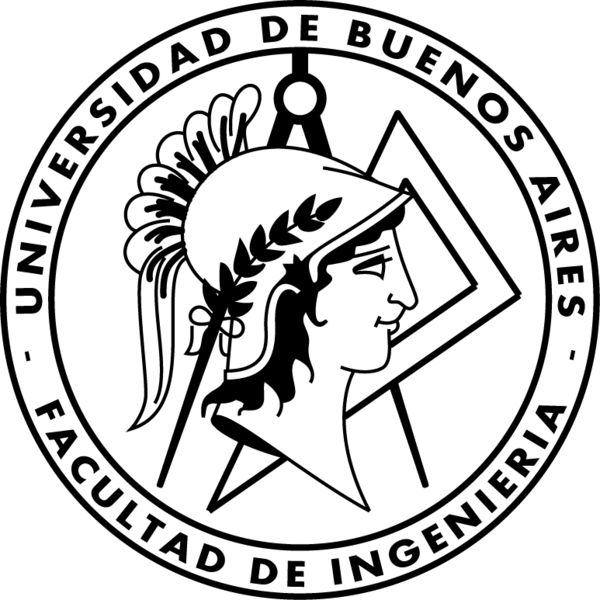
\includegraphics{images/logofiuba.png}\\[1cm]
\textsc{\Large Universidad de Buenos Aires}\\[1cm]
\textsc{\large Facultad de Ingeniería}\\[1.5cm]
\textsc{\LARGE 75.33 - Introducción a los Sistemas Distribuidos}\\[0.5cm]
    \Large Trabajo Practico
    \\[0.2cm]

    \vskip 2cm
    
    \begin{tabular}{l c r}
    \hline
    \hline
    \large{Nombre} & \hspace{10mm}{Padrón} & 
    \hspace{10mm}{Mail}\\
    \hline
    \hline
    \large{Gamberale, Luciano Martin}&\hspace{10mm}105892 & \hspace{10mm}{lgamberale@fi.uba.ar}\\
    \large{Martínez Quintero, Erick} & \hspace{10mm}103745 &
    \hspace{10mm}{egmartinez@fi.uba.ar}\\
    \large{Monpelat, Facundo}&\hspace{10mm}92716 & \hspace{10mm}{fmonpelat@fi.uba.ar}\\
    \large{Vasquez Jimenez, Miguel Angel}&\hspace{10mm}107378 & \hspace{10mm}{mvasquezj@fi.uba.ar}\\
    \large{Guglielmone, Lionel}&\hspace{10mm}96963 & \hspace{10mm}{lguglielmone@fi.uba.ar}\\
    \hline
    \hline
\end{tabular}

\large{ }   


\vfill

\end{titlepage}
\tableofcontents
\newpage


\section{Introducción}

En el siguiente informe se describe el diseño e implementación de:

\begin{itemize}
    \item Una arquitectura de aplicación cliente-servidor para la transferencia de archivos
    \item Una implementación de protocolo RDT (Reliable Data Transfer) empleando UDP de base, extendiéndolo con técnicas de control de flujo y control de errores.  
\end{itemize}

La solución se desarrolló con la finalidad de brindar una transferencia de datos confiable y eficiente entre dispositivos en una red de computadoras, simulada con \textbf{Mininet}.

La arquitectura implementada se basa en los principios de la arquitectura cliente-servidor, en la que el cliente envía solicitudes al servidor y el servidor responde con los recursos solicitados. Para lograr esto, se utilizaron \textit{sockets} en \textbf{Python} para implementar la comunicación entre los distintos hosts.

Durante la implementación, se encontraron dificultades en el manejo de paquetes y segmentos, así como en la coordinación del \textit{time out} para garantizar la correcta transferencia de los archivos. Para superar estos desafíos, se aplicaron técnicas de control de flujo y control de errores. Específicamente, se utilizaron las técnica de \textbf{Stop-and-wait} y \textbf{Selective Repeat} para controlar el flujo de datos y emplear manejo de los errores de transmisión.

Con el fin de evaluar el rendimiento de la arquitectura implementada, se utilizó Wireshark para observar diferentes métricas de red y analizar el tráfico de paquetes.

Este trabajo toma como base los conceptos presentados en el libro \textit{Computer Networking: A Top-Down Approach}, de Kurose y Ross, séptima edición, en el que se describen los diferentes aspectos de las redes de computadoras y los protocolos utilizados en ellas. Asimismo, se utilizaron las notas de las clases. La implementación de esta solución no solo permitió poner en práctica los conceptos aprendidos, sino que también permitió aplicarlos a un problema real en el mundo de las redes de computadoras.

\newpage

\section{Hipótesis y suposiciones realizadas}

\paragraph{Suposiciones}
\begin{itemize}
    \item Los clientes tienen acceso a una red con suficiente ancho de banda para la transferencia de archivos (el desarrollo está en un ámbito controlado)
    \item Los servidores tienen suficiente capacidad de almacenamiento para los archivos que se subirán (el desarrollo está en un ámbito controlado)
    \item Los clientes y servidores tienen un sistema operativo que soporta los \textit{sockets} y el protocolo de transporte UDP
    \item Los clientes y servidores pueden resolver nombres de host utilizando servicios de DNS.
    \item Los tamaños de archivo no son tan grandes como para agotar el espacio en disco disponible en el servidor (se define un límite máximo para las transferencias)
    
\end{itemize}

\paragraph{Hipótesis}
\begin{itemize}
    \item Los clientes tienen los permisos necesarios para acceder a los archivos que quieren subir o descargar
    \item El cliente y el servidor utilizan los mismos algoritmos de control de flujo y errores (Stop-and-wait o Selective Repeat) y temporizadores (\textit{timeout})
    \item No hay restricciones de seguridad en la red que puedan afectar la transferencia de archivos, como \textit{firewalls} o filtrado de paquetes
    
\end{itemize}

\newpage

\section{Implementación}

Para el protocolo de transporte se utilizo el \textit{header} llamado HeaderRDT, conformado de los siguientes campos:
\begin{enumerate}
    \item Protocol: 1 byte - Selecciona el protocolo
    \begin{itemize}
        \item SAW = 0
        \item SR = 1
    \end{itemize}
    \item Data Size: 4 bytes - Denota el tamaño de los datos
    \item Seq Number: 4 bytes - Numero de secuencia del paquete
    \item Ack Number: 4 bytes - Acuso de recibo del paquete
    \item Syn: 1 byte - Bit de sincronización
    \item Fin: 1 byte - Bit de finalización
    \item Header Checksum: 1 byte - Numero validador CRC de la integridad del \textit{header}
\end{enumerate}

Siguiendo con el protocolo de aplicación se utilizo el \textit{header} llamado ApplicationHeaderRDT, donde los campos son:
\begin{enumerate}
    \item Transfer Type: 1 byte - Selecciona la transferencia
    \begin{itemize}
        \item Upload = 0
        \item Download = 1
    \end{itemize}
    \item File Name: 40 bytes - Nombre de archivo
    \item File Size: 4 bytes - Tamaño de archivo
    \item Header Checksum: 1 byte - Numero validador CRC de la integridad del header
\end{enumerate}

Se puede ver en la siguiente imagen como se conforma un segmento completo con ambos \textit{headers} y datos de aplicación:

\begin{figure}[H]
    \centering
    \begin{center}
    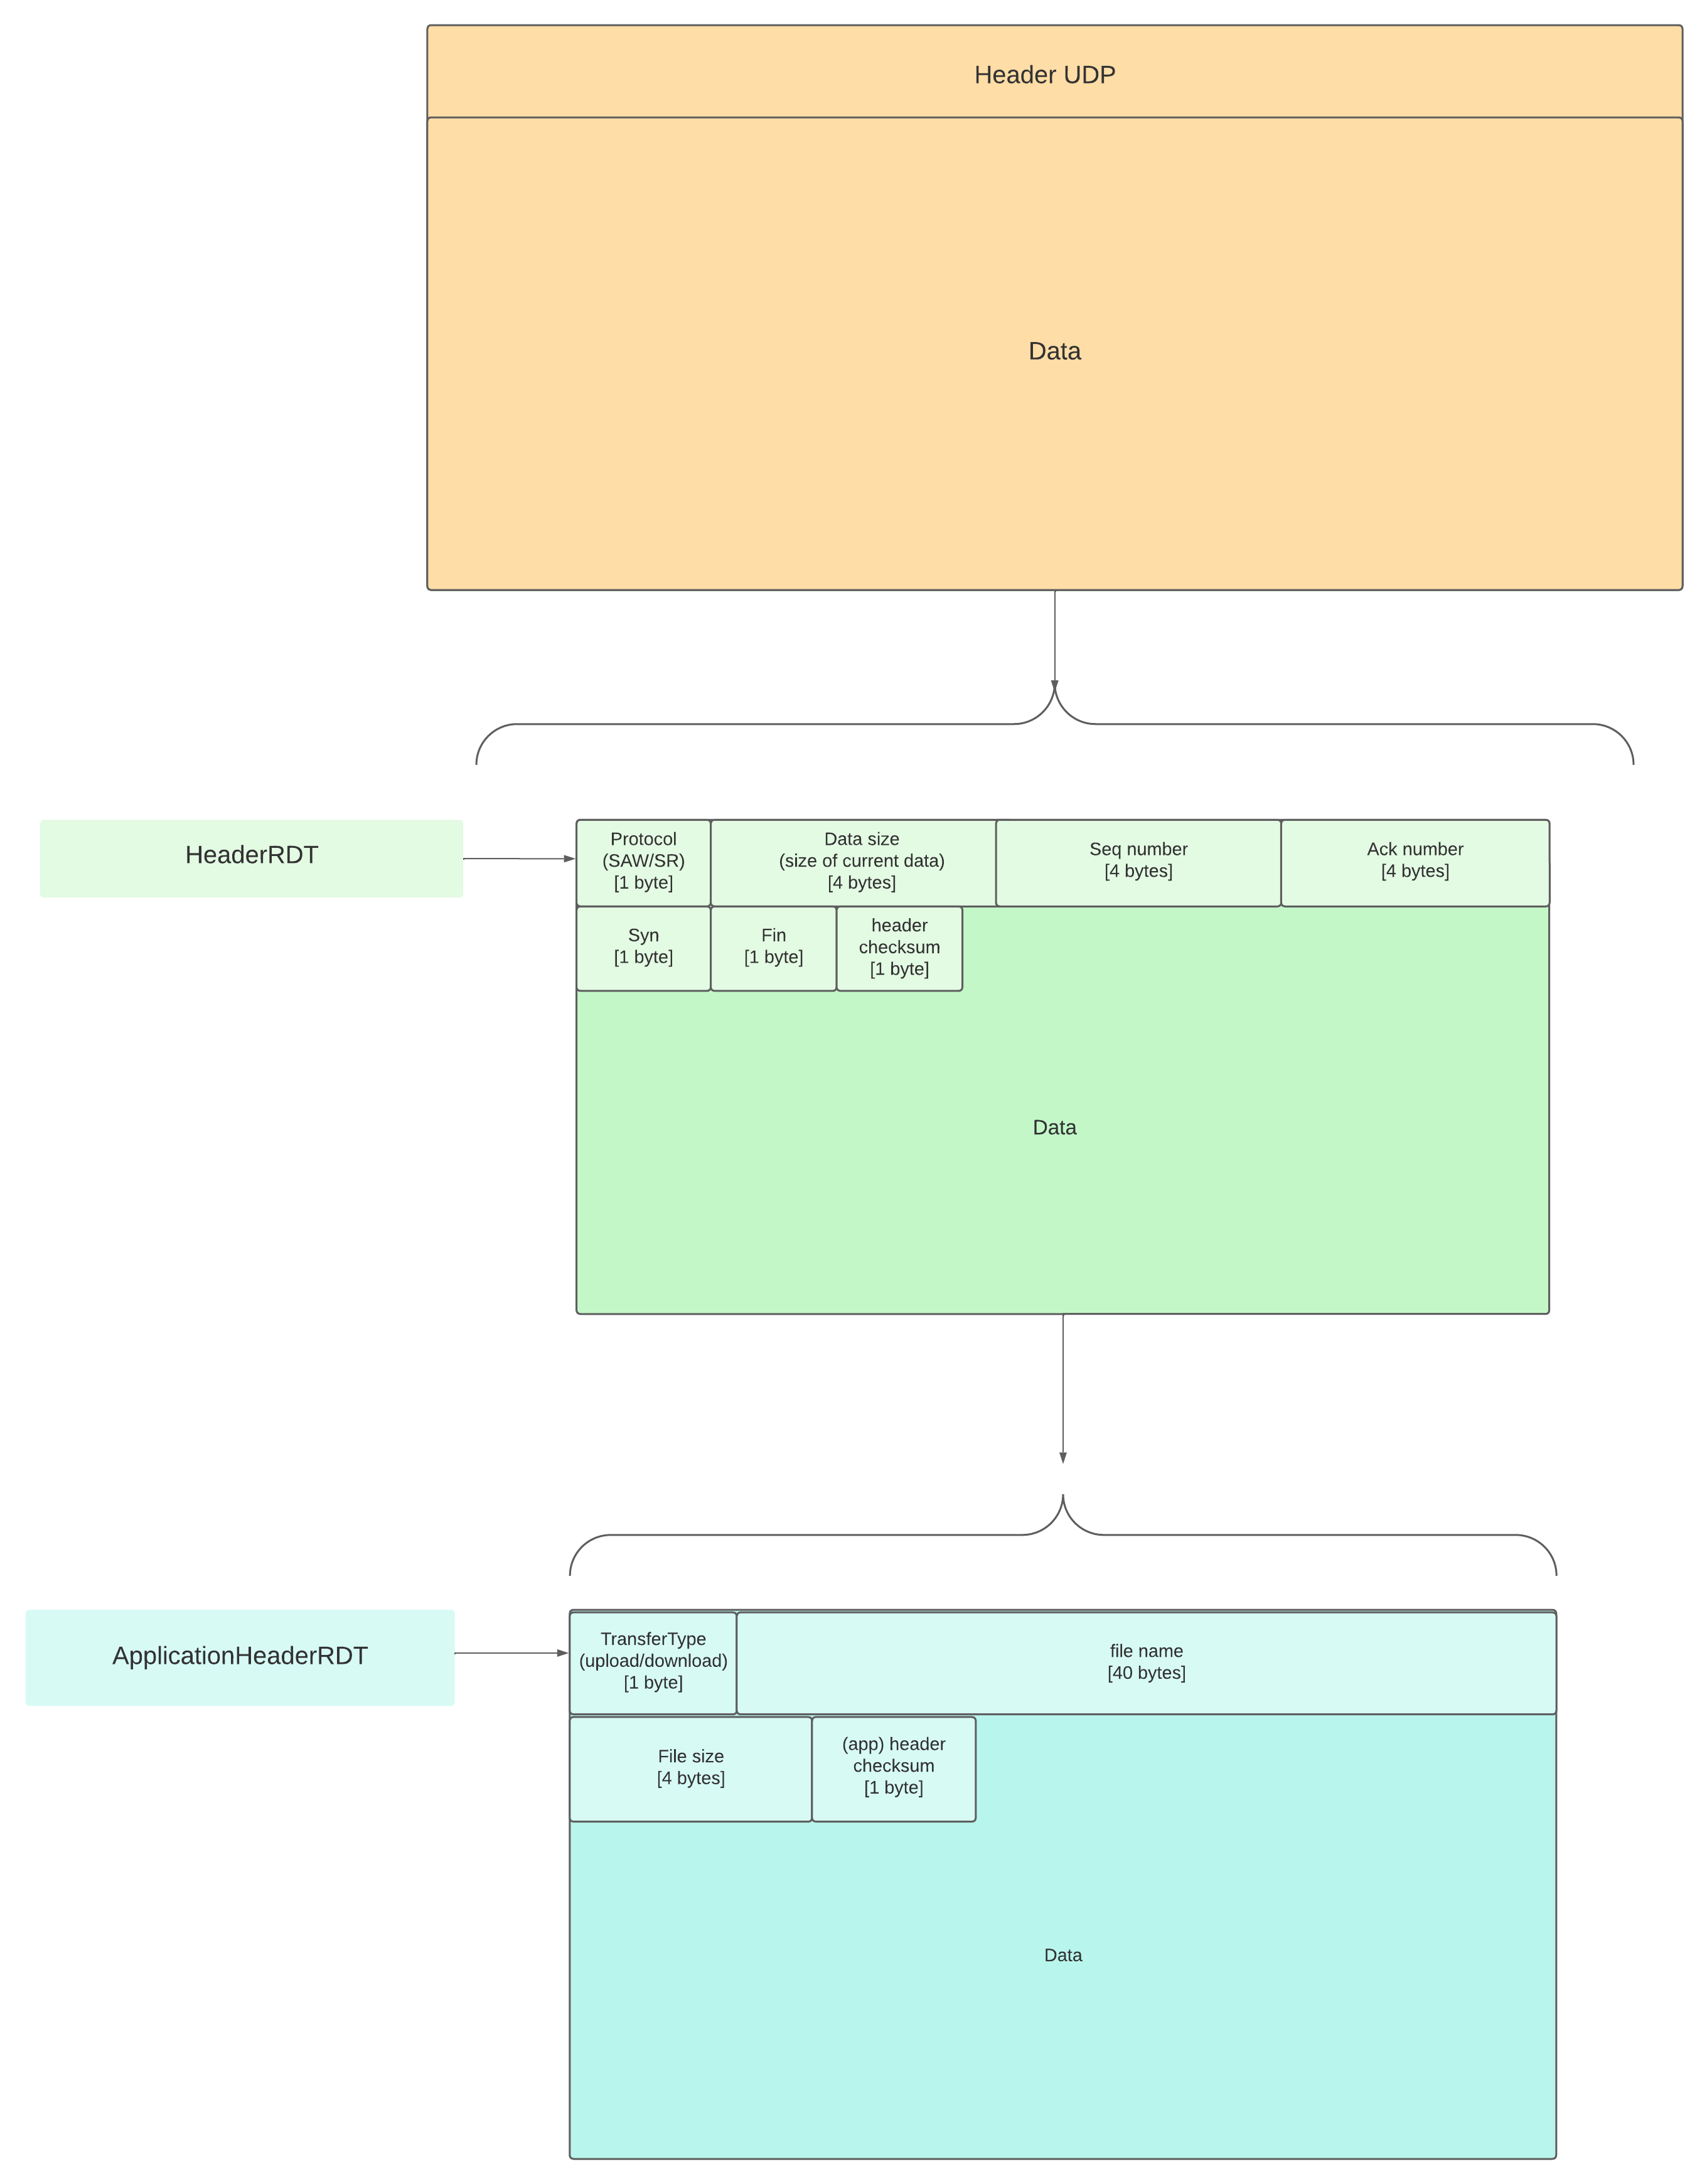
\includegraphics[width=16cm]
    {images/implementacion/Segments_Architecture.png}
    \end{center}
    \caption{Arquitectura de los segmentos Headers mas Datos}
\end{figure}

\newpage

En general, para la realización del \textit{three-way-handshake} se implementó un protocolo de envío y recepción de forma tal que se realizan múltiples reintentos de conexión, esto dado a que definimos que ambos hosts reciban al menos un mensaje de tipo \textit{handshake} como condición necesaria para que el cliente establezca una conexión. Si bien se envía un tercer mensaje de confirmación desde el cliente (como se muestra en la figura de la siguiente página), el servidor puede optar por recibir data de usuario directamente tras haber recibido el primer mensaje. Esto hace que se contemple el eventual caso en el que se pierda el ultimo paquete de confirmación del \textit{handshake}, y funcione de manera eficiente.

Luego, para implementar los protocolos de aplicación se definieron las siguientes secuencias de mensajes a interpretar por cada uno de los hosts:

\begin{itemize}
    \renewcommand\labelitemi{$->$}
    \item \textbf{Caso: Cliente solicita descarga} \\
    Para este caso se definió el envió obligatorio del objeto $"ApplicationHeaderRDT"$, particularmente requiriendo ida y vuelta (Cliente $->$ Server  y Server $->$ Cliente), de tal forma que el cliente pueda obtener información sobre el estado del archivo que quiere descargar (dado que el mismo solo conoce el nombre del archivo a priori). En la respuesta recibida por el servidor puede obtener:
    \begin{itemize}
        \item Confirmación de que va a enviarle el archivo si se reemite el ApplicationHeader con el mismo filename y si se le brinda un filesize no nulo.
        \item Rechazo del pedido (porque el archivo no existe en el server), en donde se le envía el ApplicationHeader con NO SUCH FILE de filename y valor nulo de filesize.
    \end{itemize}
\end{itemize}

En la siguiente página se observa un gráfico del inicio de la comunicación recién descrita:
(Para simplificar la visualización se muestra el caso mencionado utilizando Stop And Wait)

\newpage

\begin{figure}[H]
    \centering
    \begin{center}
    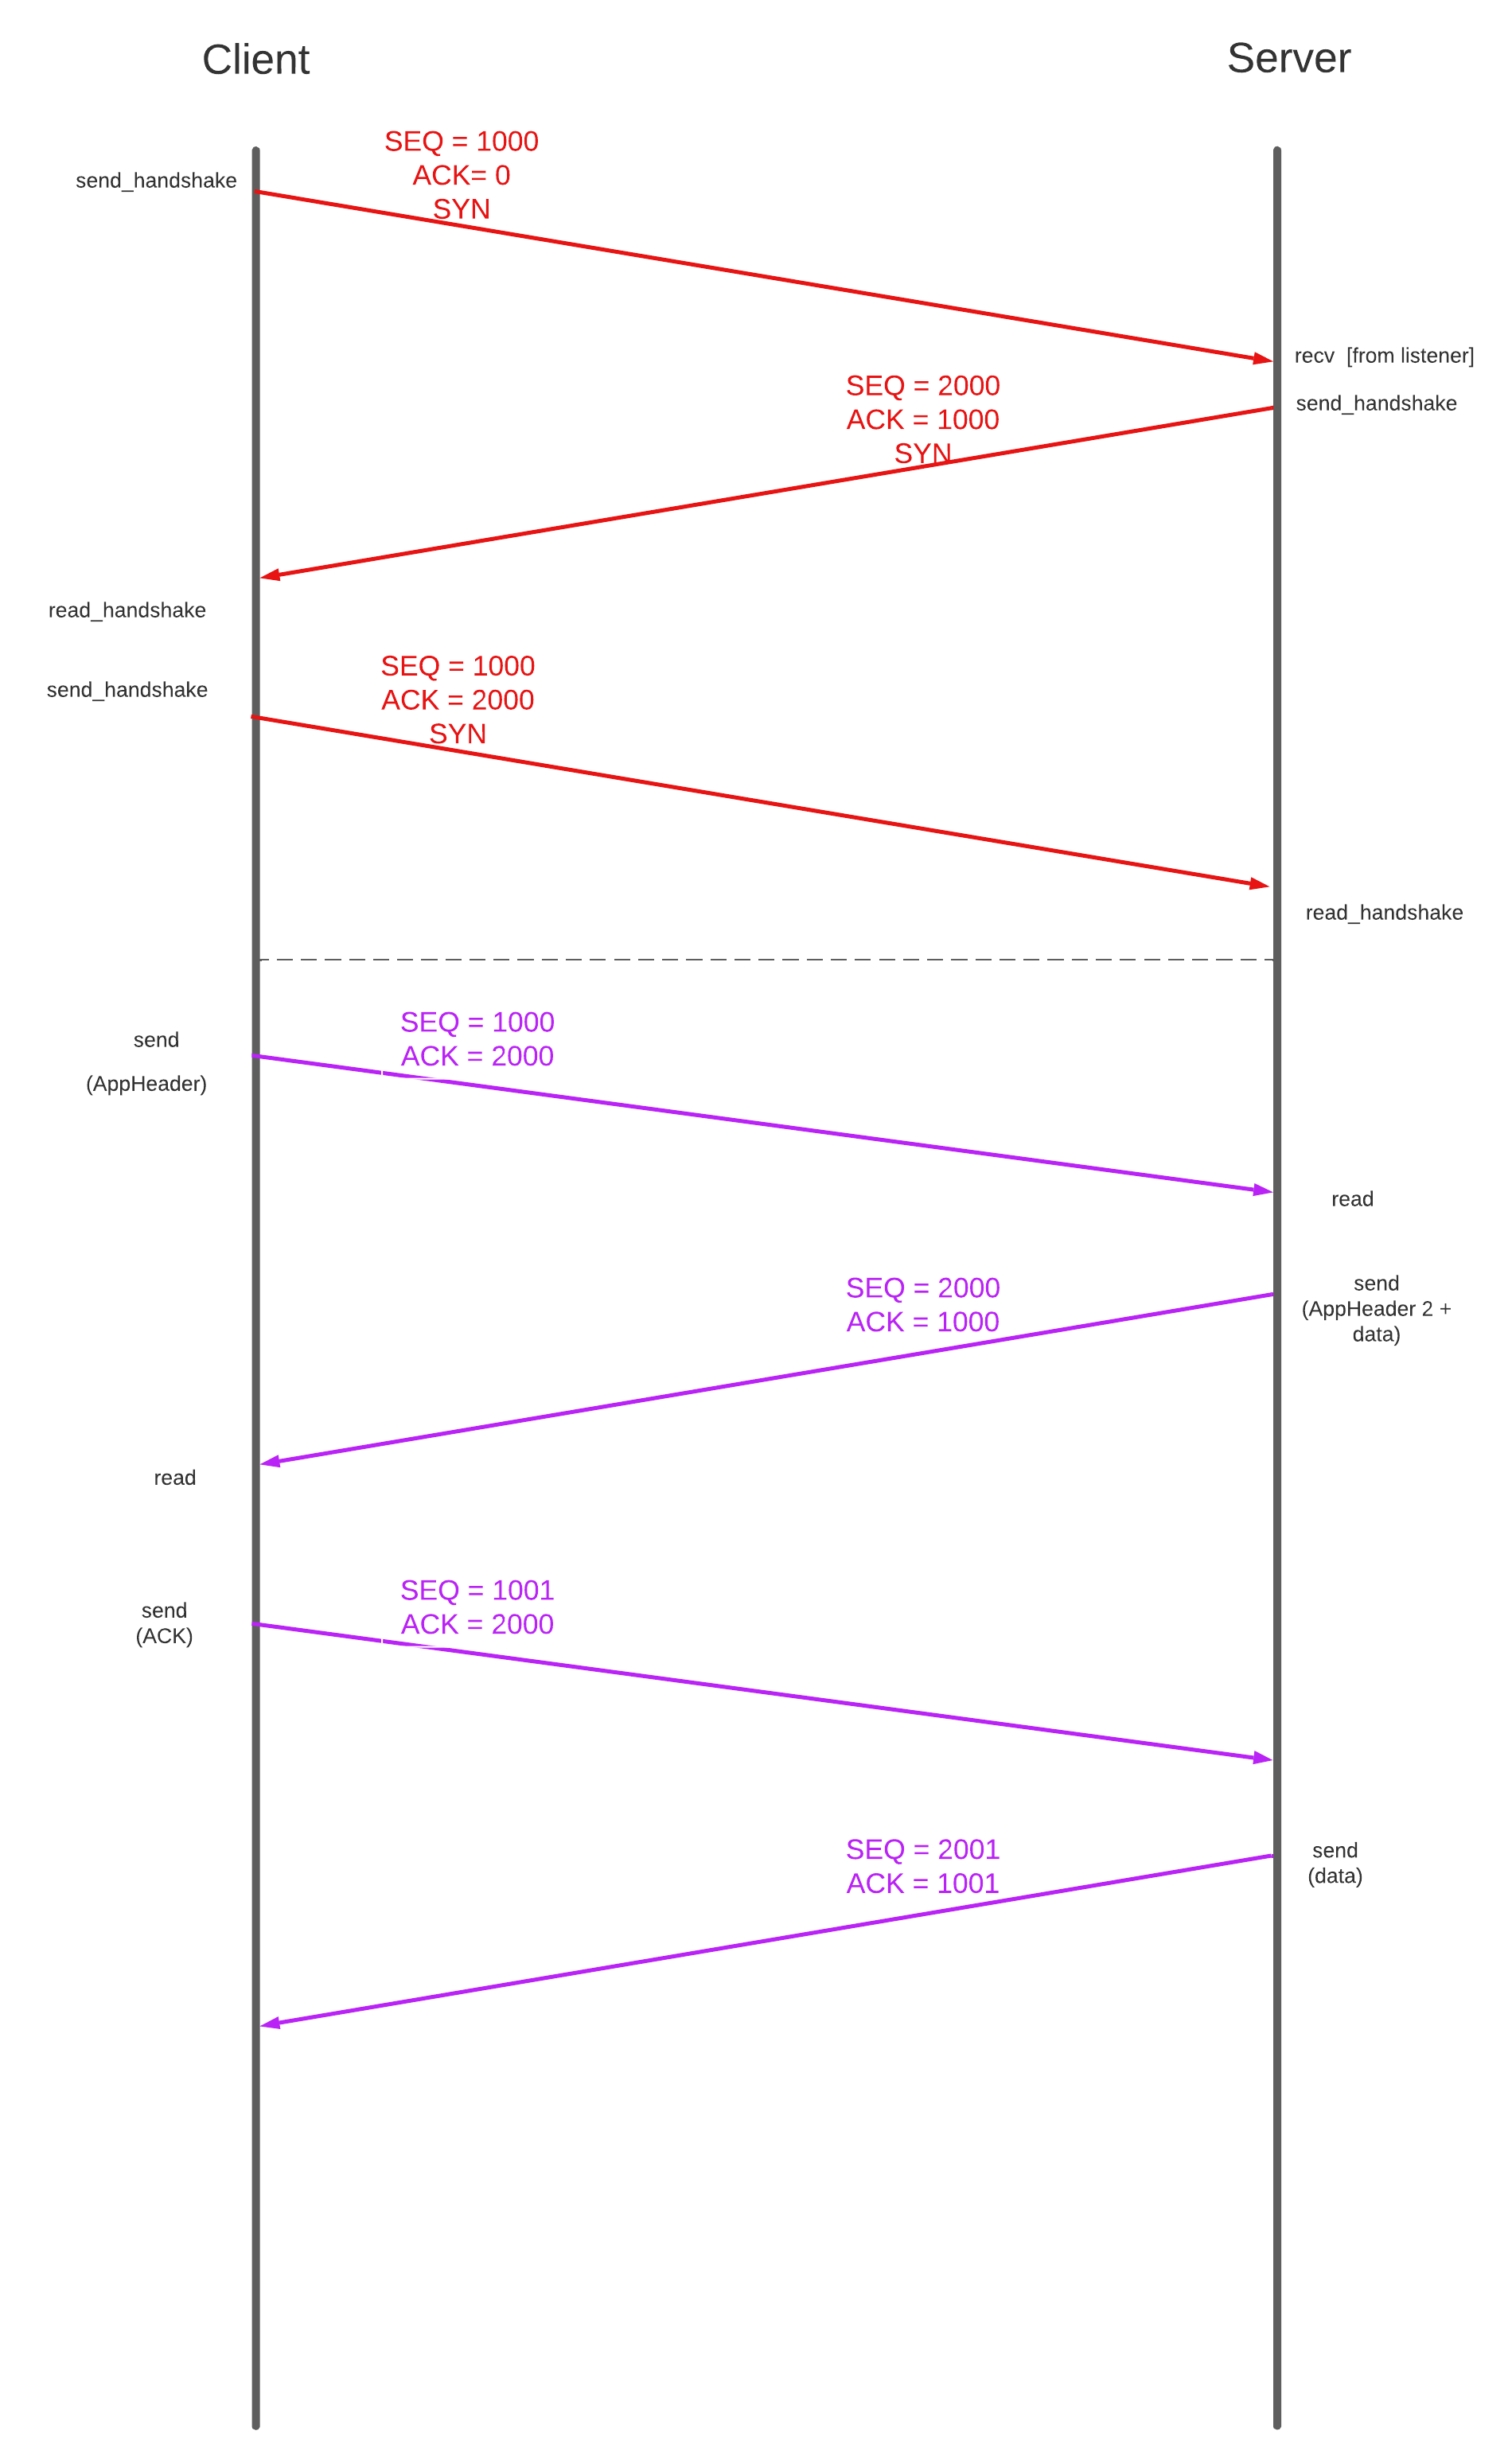
\includegraphics[width=13cm]
    {images/implementacion/comunicacion_general_SAW_download.png}
    \end{center}
    \caption{Comunicación Cliente-Servidor Stop and Wait Download}
\end{figure}

\newpage

\begin{itemize}
    \renewcommand\labelitemi{$->$}
    \item \textbf{Caso: Cliente solicita subida} \\
    Para este caso se definió el envió del objeto $"ApplicationHeaderRDT"$, requiriendo solo ida (Cliente $->$ Server), de tal forma que el cliente pueda avisar al server sobre la información del archivo que quiere subir. En la respuesta recibida por el servidor puede obtener:
    \begin{itemize}
        \item Confirmación de que puede subir el archivo (por medio de un mensaje sin data, solo con el HeaderRDT para representar un ACK).
        \item Rechazo del pedido de subida (en caso de que el archivo exceda el tamaño máximo de almacenamiento permitido por el server, definido arbitrariamente como 500 MiB).
    \end{itemize}
\end{itemize}

En la siguiente página se muestra el comienzo de la comunicación del caso recién descrito:

\newpage

\begin{figure}[H]
    \centering
    \begin{center}
    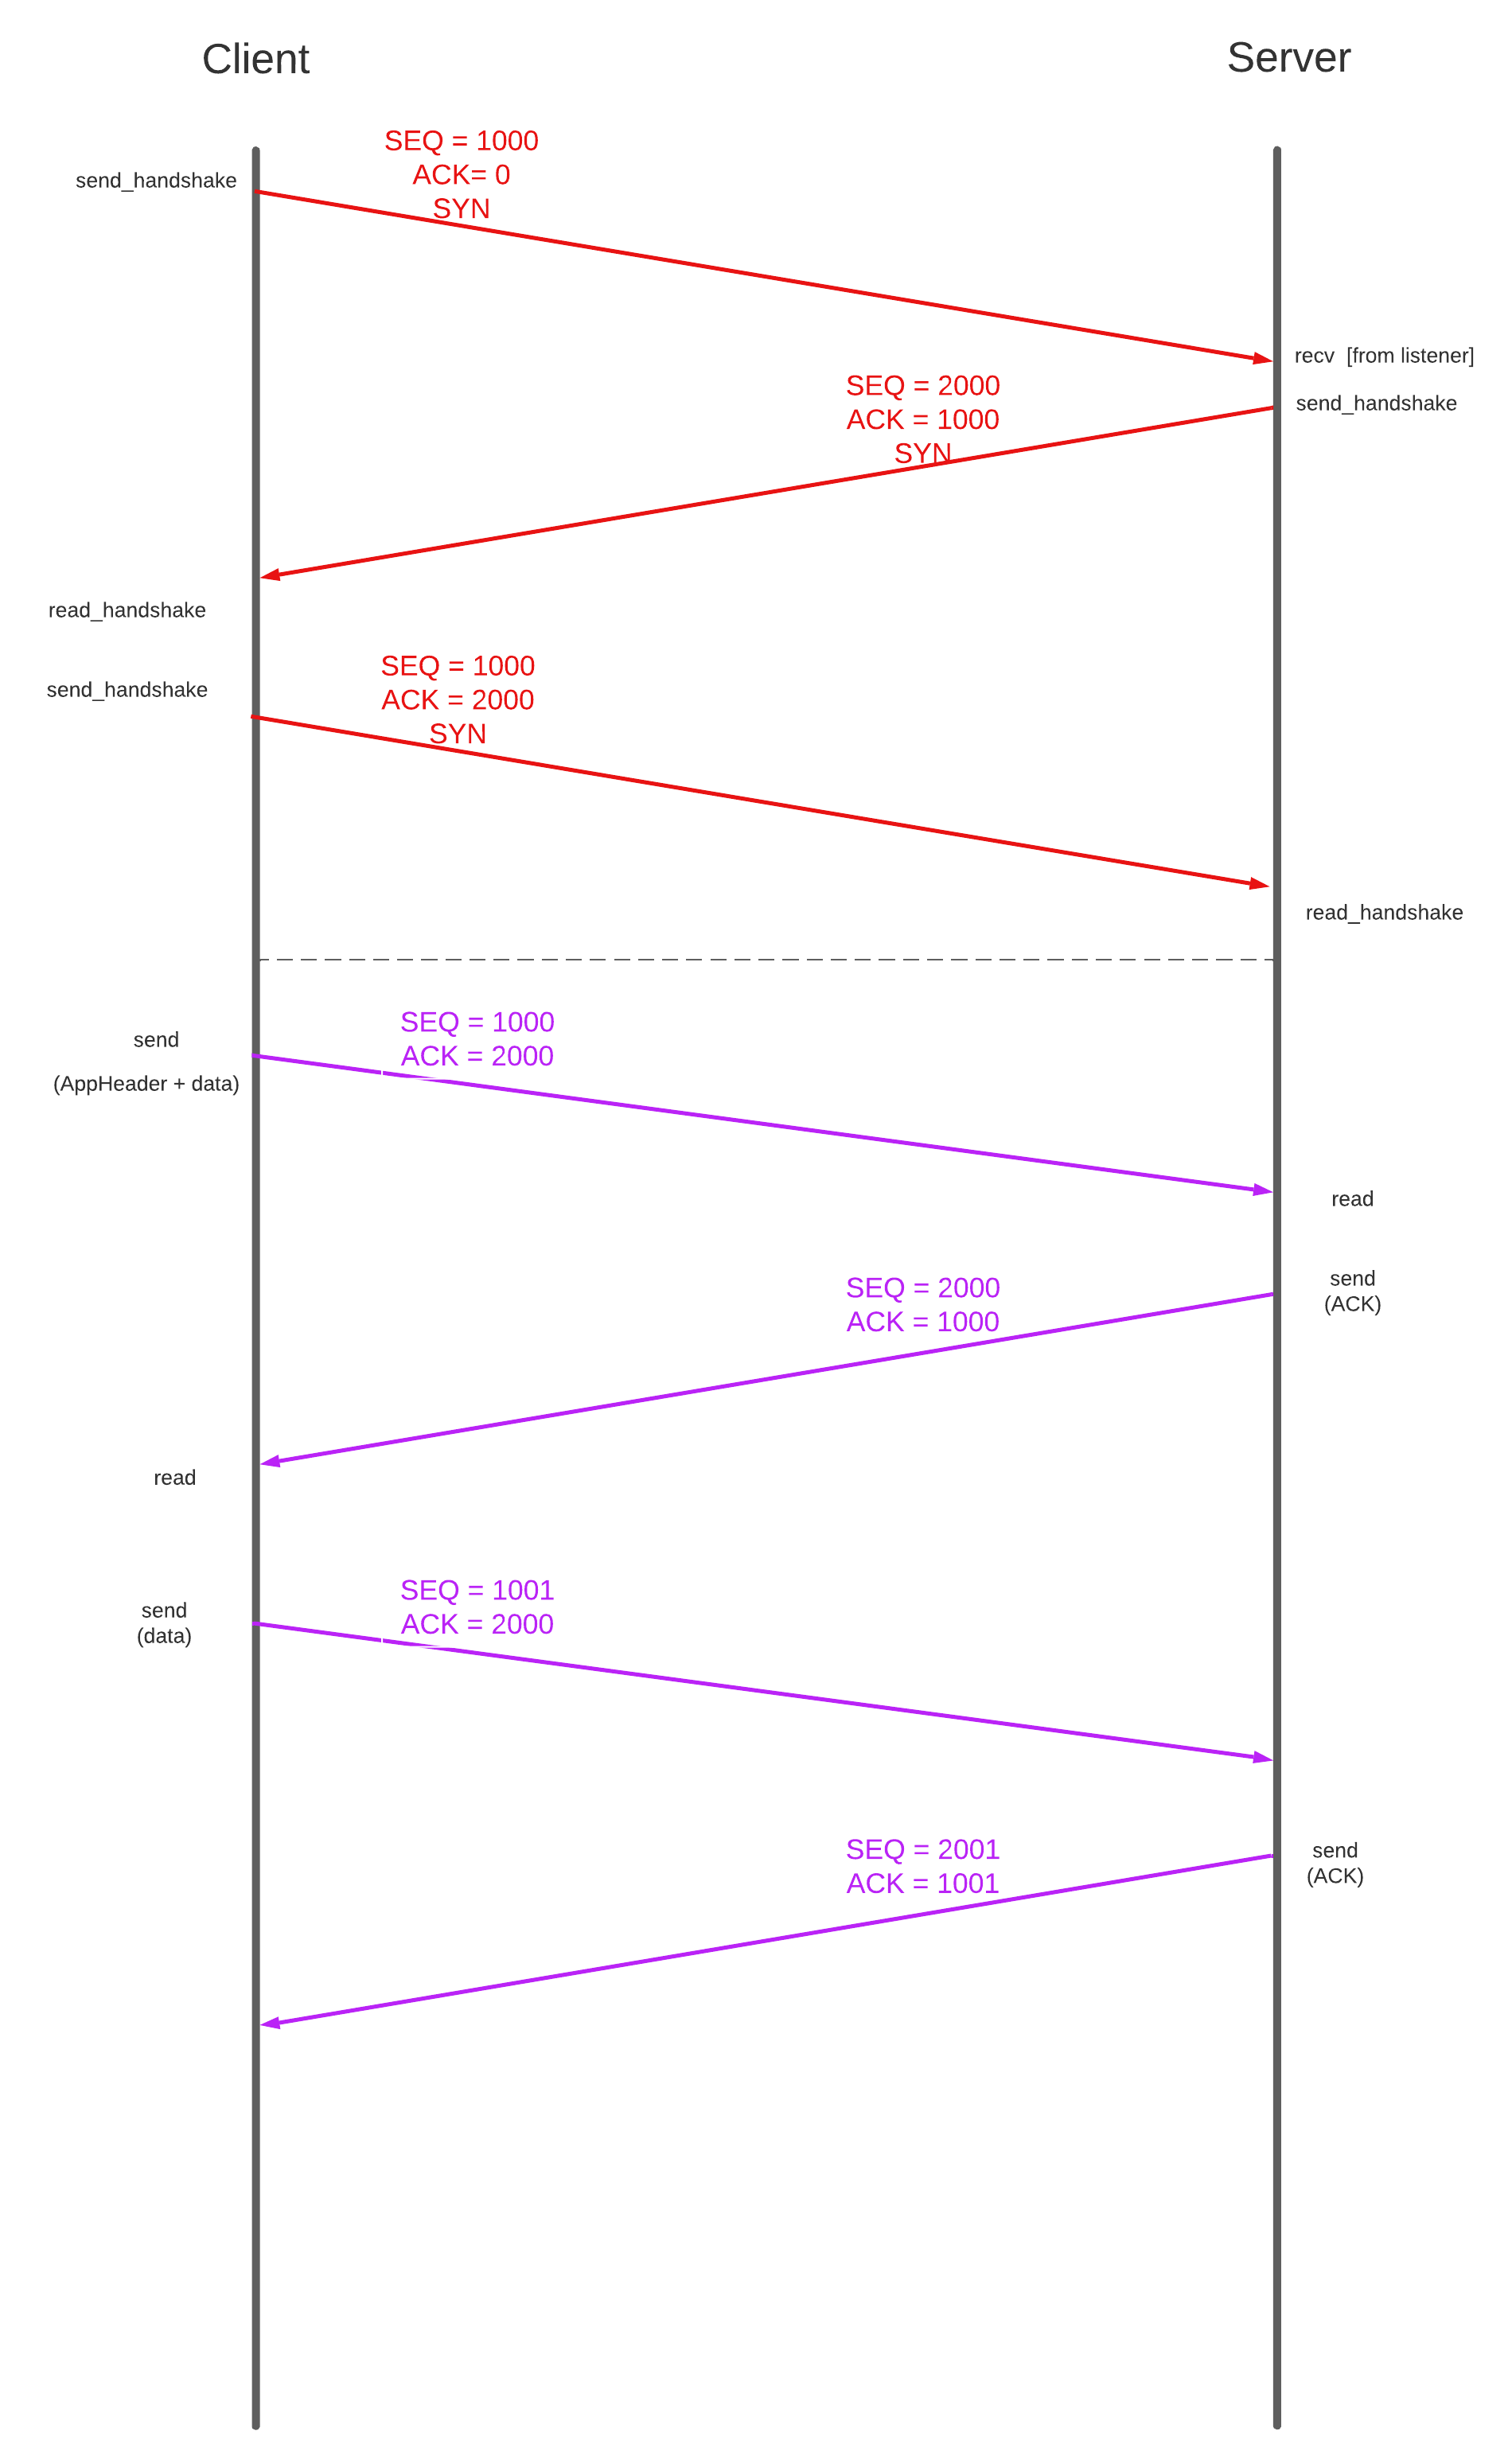
\includegraphics[width=13cm]
    {images/implementacion/comunicacion_general_SAW_upload.png}
    \end{center}
    \caption{Comunicación Cliente-Servidor Stop and Wait Upload}
\end{figure}

\newpage

A continuación se detalla la implementación de una de las secciones más importante del desarrollo del protocolo: El manejo de envío de paquetes por medio de Selective Repeat.

Dicho protocolo se implementó por medio del modelado de una SlindingWindow encargada de mantener información del estado de una cantidad fija de paquetes que puede ser enviada, por medio del almacenamiento de sus correspondientes sequence numbers locales, ack numbers, y una lista con registros para identificar si determinado paquete contenido en la window ya fue enviado o si ya se recibió su correspondiente mensaje ACK. 

La secuencia de envío se hace de tal forma que se pueden enviar de forma eficiente los paquetes contenidos en la window actual, realizando una recepción (read) no bloqueante por cada uno de dichos envíos. 

De esta forma se pueden continuar recibiendo ACKs dinámicamente, y la window se va a "desplazar" en el caso en el que su paquete contenido de menor sequence number ya se haya informado como recibido por el host contrario. 

Finalmente, si se agotan los posibles envíos de la window (es decir, si para la window actual ya se enviaron todos los paquetes pero aún no se recibió el ACK necesario para desplazarla), se procede a realizar una recepción bloqueante (con un timeout y cierta cantidad de reintentos en caso del mismo) para permitir la recepción de posibles ACKs que aun no hubiesen llegado. 

Si se da el caso de timeout se procede a reenviar selectivamente los paquetes que no se hayan confirmado como recibidos por el host contrario (ya sea porque se perdieron dichos paquetes o porque se hayan perdido los correspondientes ACKs. En este último caso si se llegan a obtener paquetes replicados simplemente son descartados por el host que corresponda). 

De esta forma no solo se garantiza el envío confiable de paquetes en situaciones con packet loss, sino que tambien se tiene en cuenta la eficiencia al enviar selectivamente los paquetes necesarios a retransmitir en caso de perdidas. 


En la siguiente página se muestra un gráfico ilustrativo de la comunicación anterior:

\newpage

\begin{figure}[H]
    \centering
    \begin{center}
    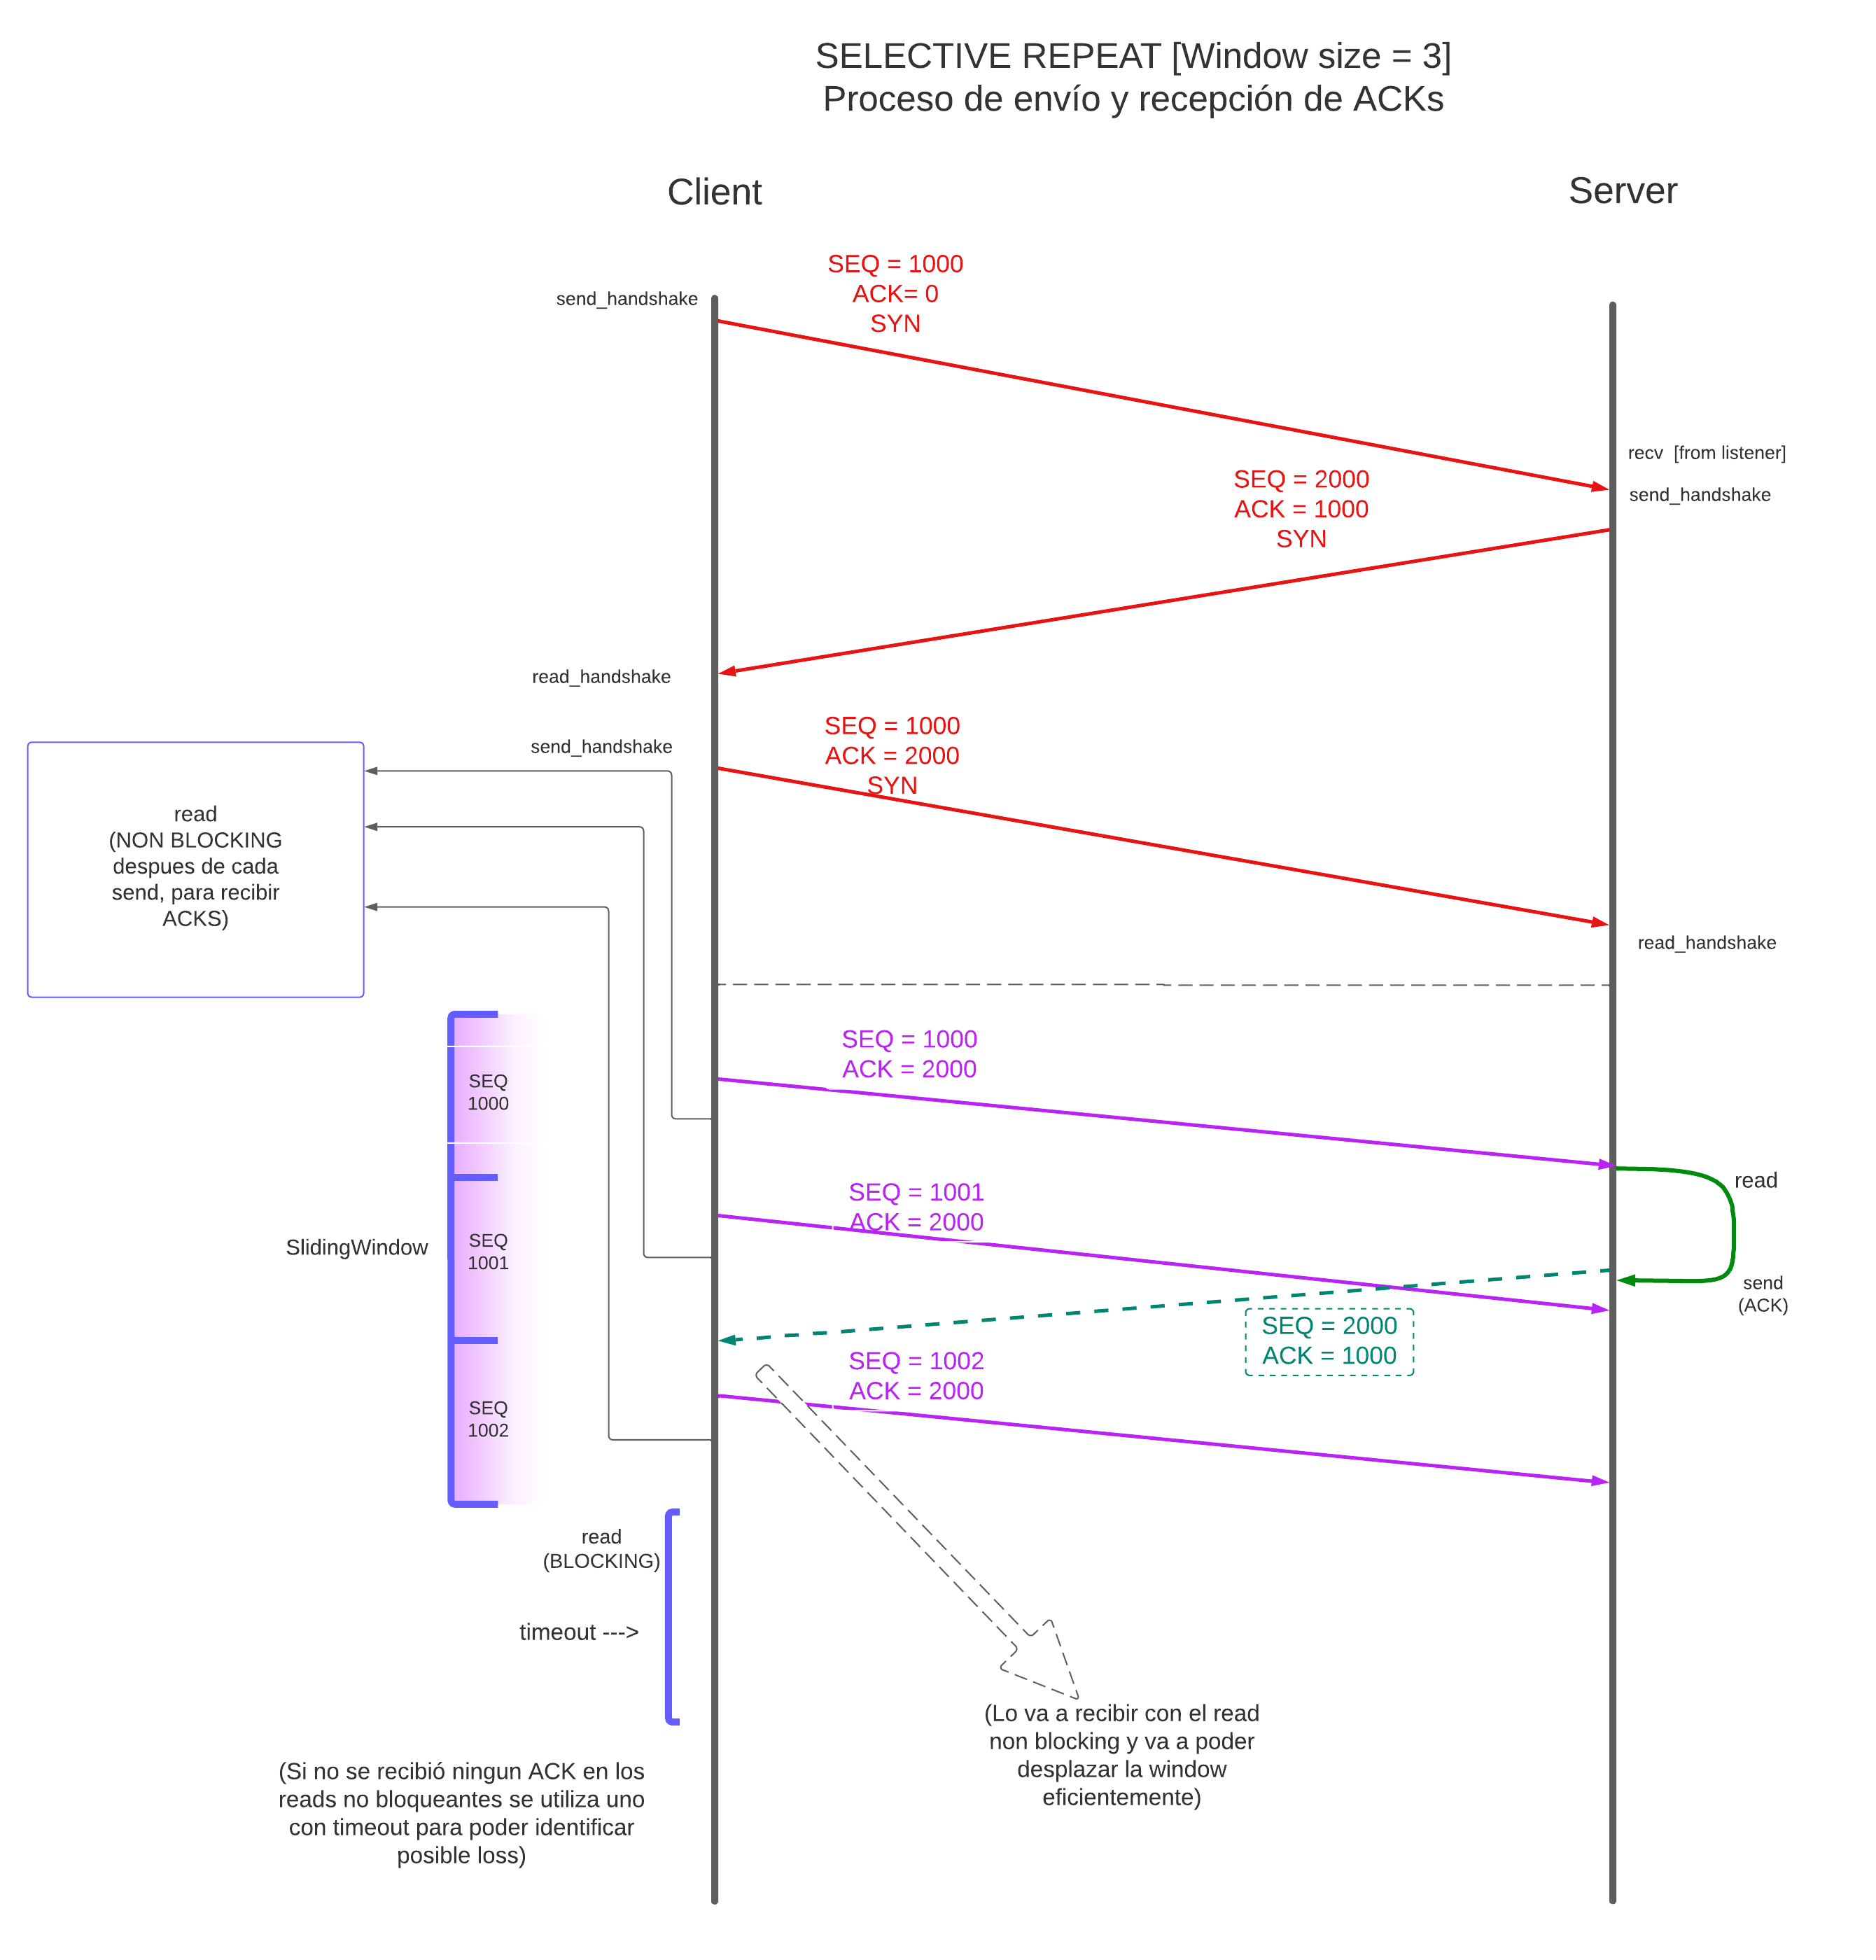
\includegraphics[width=17cm]
    {images/implementacion/Proceso_send_and_recv_de_ACKs_SRepeat.png}
    \end{center}
    \caption{Comunicación Cliente-Servidor Stop and Wait Upload}
\end{figure}

\newpage

\textbf{Notas adicionales de la implementación} \\
\begin{itemize}
    \item \textbf{Implementación de los streams de conexión} \
    Una parte importante del desarrollo del programa fue el modelado e implementación de las entidades ListenerRDT, AccepterRDT y StreamRDT.
    Como se esperaría (tomando como ejemplo a las conexiones TCP), el rol del Listener es poder escuchar intentos de comunicación entrantes. Posteriormente el Accepter se encarga de culminar el establecimiento de conexión por medio de la creación de una instancia de StreamRDT para tener un canal de comunicación directa con el cliente particular que solicitó la conexión. Luego, el Stream es el ente más importante ya que se debe encargar del manejo completo de las transferencias de paquetes (haciendo uso de los servicios que le brinde su protocolo, sea Stop And Wait o Selective Repeat), incluyendo recepción y envío seguro de los mismos.\
    \item \textbf{Implementación concurrente del servidor} \\
    Para el desarrollo del manejo concurrente de clientes por parte del servidor, se implementó el mismo de tal forma que se crea un thread por cada recepción de intento de conexión distinto por cada cliente hasta un determinado máximo. De esta manera se pueden realizar las operaciones requeridas por cada conexión de forma completamente independiente. Esto último es facilitado por el hecho de que los clientes (para este programa particular) no requieren de comunicarse entre sí, por lo cual su comunicación es exclusiva con el servidor y su request específica. 
    \item \textbf{Stop And Wait como caso particular} \\
    Dado que nuestra implementación del manejo de packet loss y errores Selective Repeat abarca el uso de la lógica de timeouts y reintentos para el envío de multiples paquetes (dependiendo del tamaño de la window), nos resultó lógico y viable realizar la implementación de Stop and Wait como caso particular de Selective Repeat con un tamaño de window = 1. 
    \item \textbf{Utilización de librerías} \\
    Si bien en el entorno controlado de pruebas (virtualización en Mininet) no puede llegar a darse una corrupción de bits en los paquetes transferidos, se añadió adicionalmente el uso de la librería crc de Python para corroborar la integridad de los headers pertinentes de cada paquete enviado y recibido por cada host al momento de decodificar los bits.
    \item \textbf{Wireshark Dissector} \\
    Adicionalmente se implementó un disector de Wireshark para que el programa sea capaz de interpretar el HeaderRDT que se adhiere a cada paquete transmitido por medio de nuestro protocolo. En la interpretación de cada paquete se pueden observar todos los correspondientes campos del segmento que se mencionaron anteriormente en la arquitectura de segmentos implementada. 
\end{itemize}

\newpage

\section{Pruebas}

Se toman en cuenta los siguientes casos de prueba para validación de comportamiento general (cada caso se describe por medio de la topología probada y distintos valores de \textit{packet loss}, así como secuencias de ejecución distintas):

\textbf{Nota aclaratoria}: En las pruebas mostradas a continuación se utiliza un archivo llamado $"upload$ $test"$, autogenerado con una utilidad de linea de comandos Linux. (Aclarado para no causar confusión dado que tambien se utiliza en las pruebas de downloads) El mismo tiene un tamaño al alrededor de 5 KiB.  

%%%%%%%% TOPOLOGIA 1 %%%%%%%%%%%%%%%%%%%%%%%%%%%%%%%%%%%%%%%%%%%%%%%%%%%%%%%%%%%%
Topología: Server $<->$ 1 Cliente \\
    \begin{itemize}
%%%%%%%% PACKET LOSS 0 %%%%%%%%%%%%%%%%%%%%%%%%%%%%%%%%%%%%%%%%%%%%%%%%%%%%%%%%%%%%
        \item \textbf{packet loss = 0}: (para observación del    comportamiento ideal)
            \begin{figure}[H]
                %\centering
                \begin{center}
                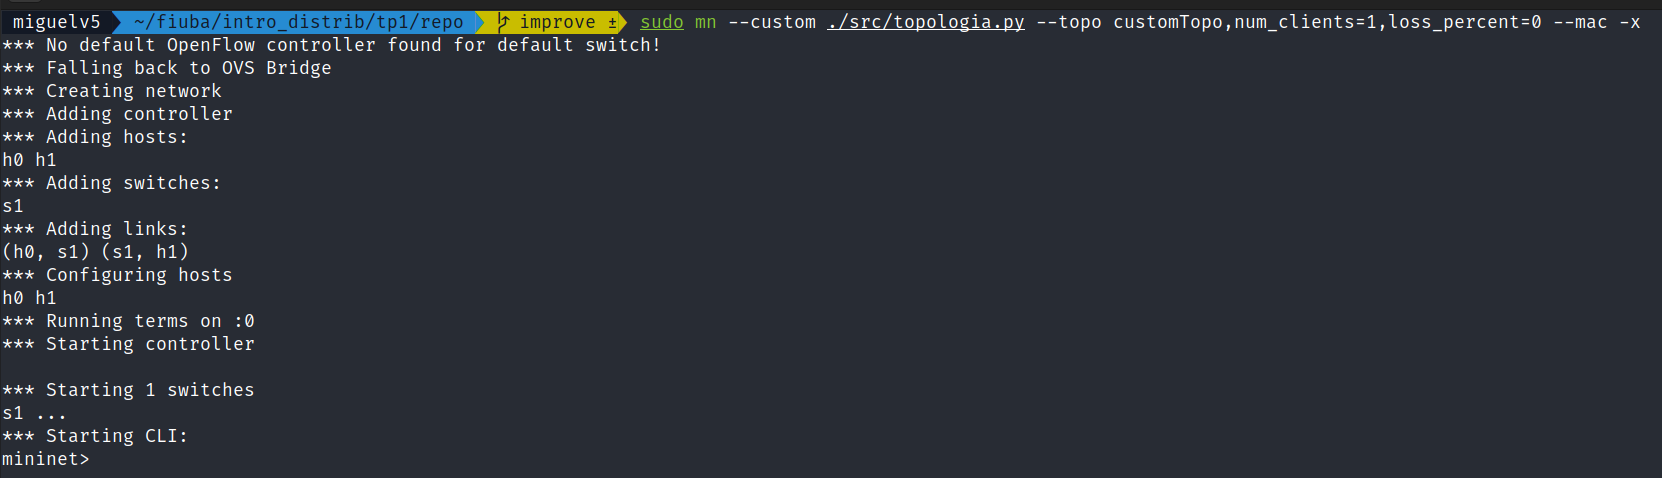
\includegraphics[width=18cm]{images/tests/t1/T1_loss0.png}
                \end{center}
                \caption{Mininet Topologia Packet loss $0\%$ }
            \end{figure}
            \begin{itemize}
%%%%%%%% UPLOAD %%%%%%%%%%%%%%%%%%%%%%%%
                \item UPLOAD del archivo (Client $-->$ Server)
                \begin{figure}[H]
                    %\centering
                    \begin{center}
                    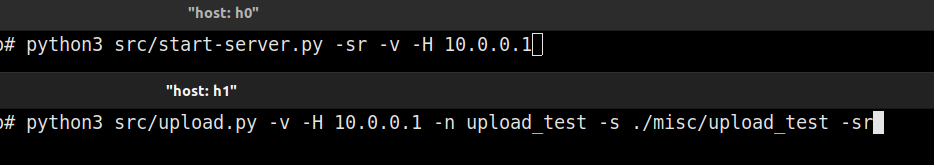
\includegraphics[width=18cm]{images/tests/t1/upload/T1_comandos_upload.png}
                    \end{center}
                    \caption{Comandos de ejecucci\'{o}n de servidor y cliente}
                \end{figure}
                \begin{figure}[H]
                    %\centering
                    \begin{center}
                    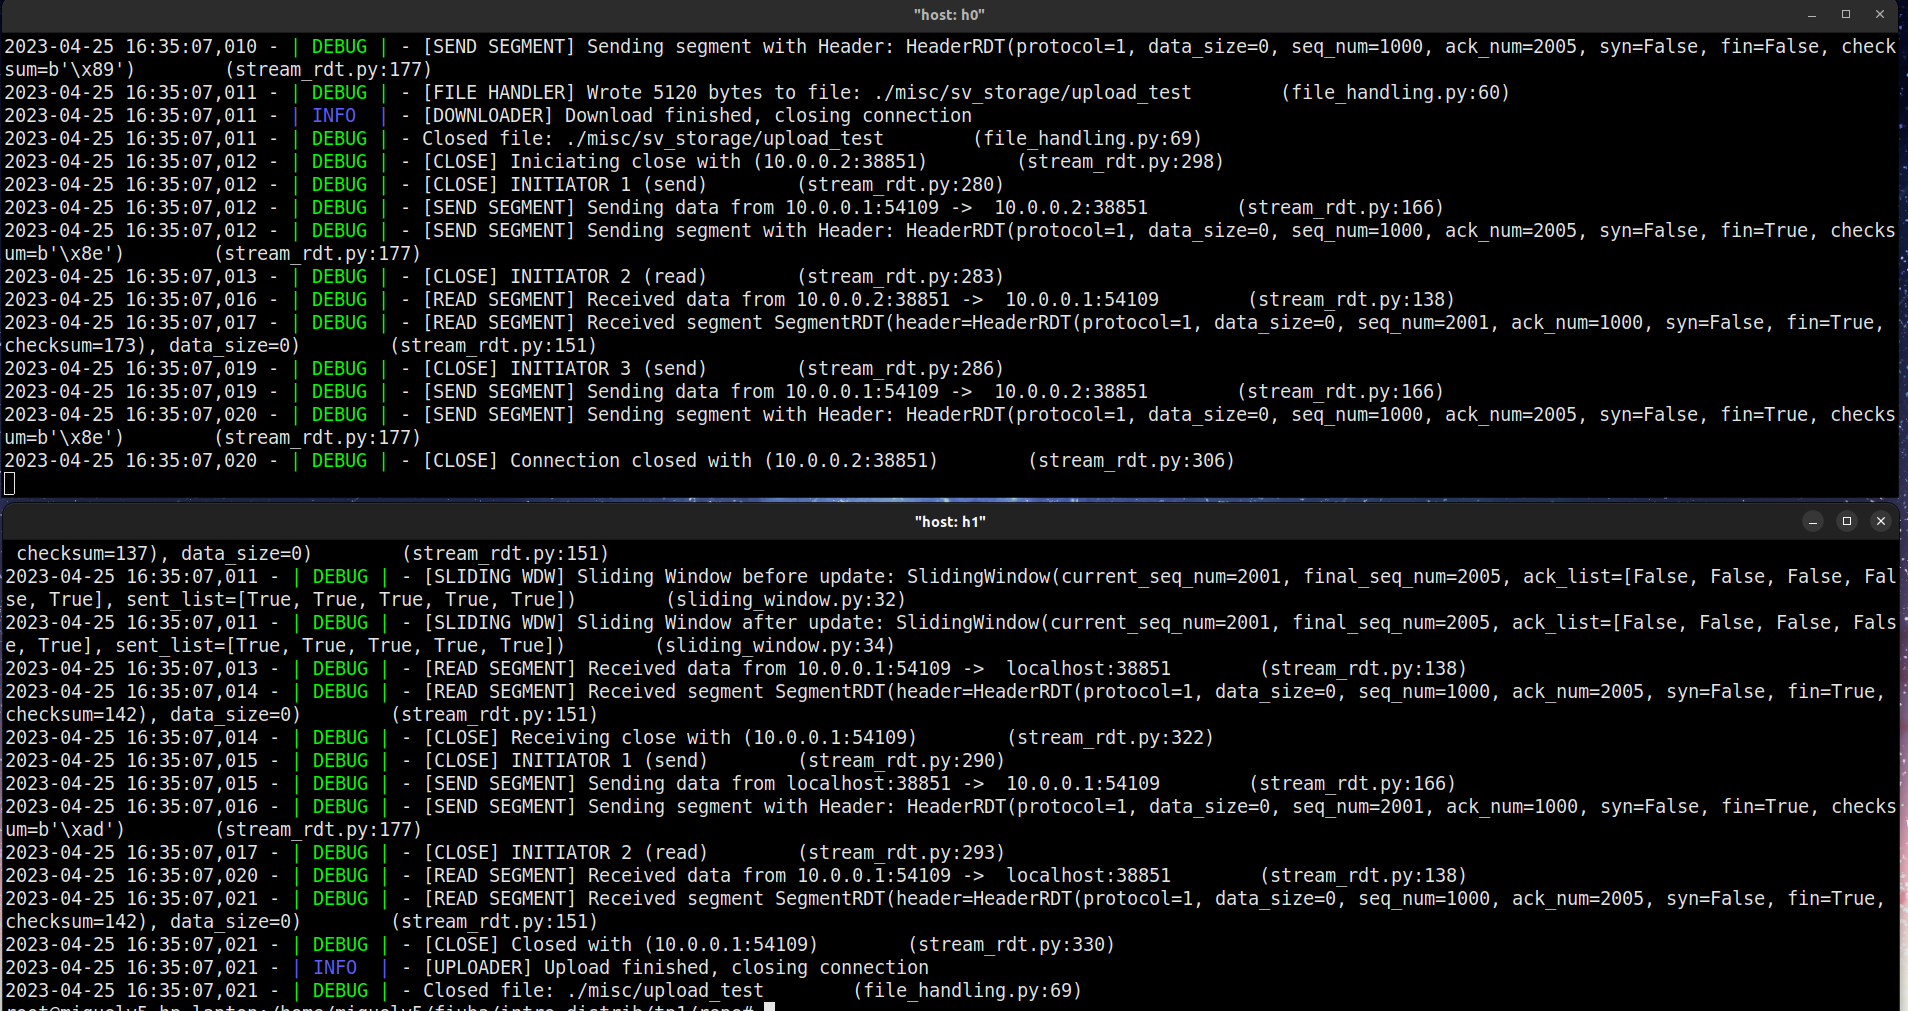
\includegraphics[width=18cm]{images/tests/t1/upload/T1_2.2_upload_SR_loss0.png}
                    \end{center}
                    \caption{Captura de comunicaci\'{o}n por linea de comandos}
                \end{figure}
                \begin{figure}[H]
                    %\centering
                    \begin{center}
                    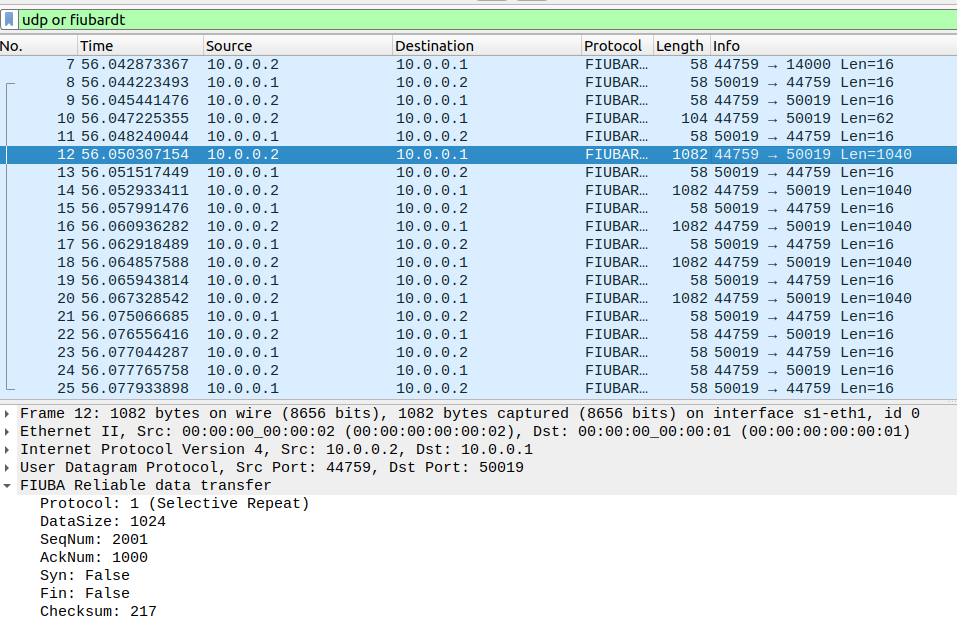
\includegraphics[width=15cm]{images/tests/t1/upload/T1_2.3_upload_SR_loss0.png}
                    \end{center}
                    \caption{Captura de wireshark del protocolo}
                \end{figure}
                \begin{figure}[H]
                    %\centering
                    \begin{center}
                    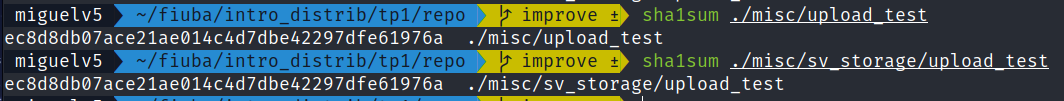
\includegraphics[width=15cm]{images/tests/t1/upload/T1_2.4_upload_SR_loss0.png}
                    \end{center}
                    \caption{Verificaci\'{o}n de SHA1 de los archivos}
                \end{figure}
%%%%%%%% DOWNLOAD %%%%%%%%%%%%%%%%%%%%%%
                \item DOWNLOAD del archivo (Client $<--$ Server)
                \begin{figure}[H]
                %\centering
                \begin{center}
                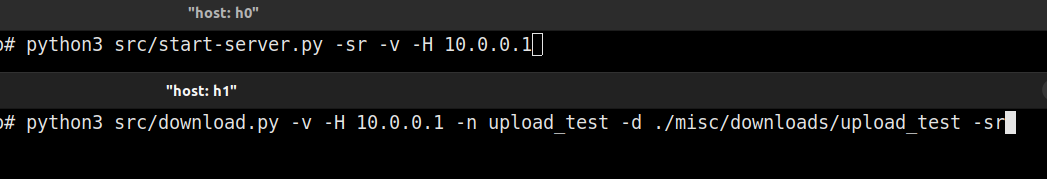
\includegraphics[width=18cm]{images/tests/t1/download/T1_comandos_download.png}
                \end{center}
                \caption{Comandos de ejecucci\'{o}n de servidor y cliente}
            \end{figure}
                \begin{figure}[H]
                    %\centering
                    \begin{center}
                    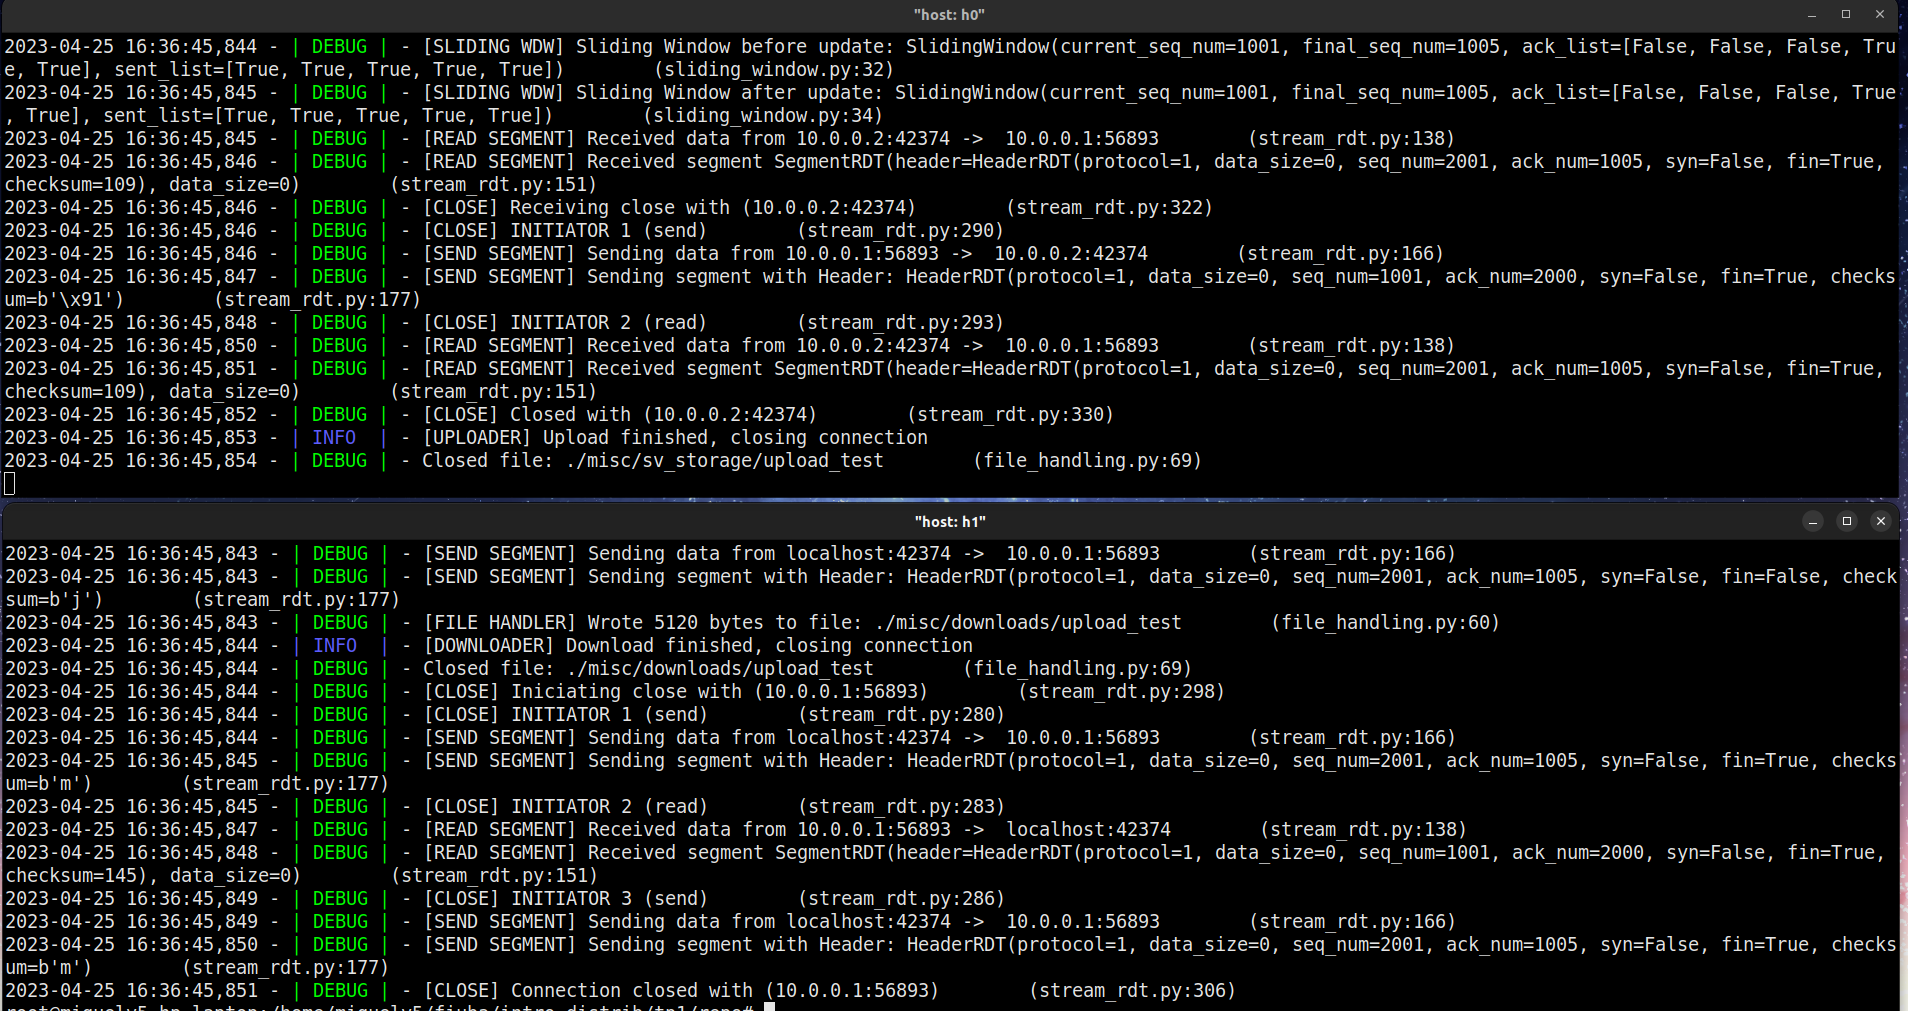
\includegraphics[width=18cm]{images/tests/t1/download/T1_3.2_download_SR_loss0.png}
                    \end{center}
                    \caption{Captura de comunicaci\'{o}n por linea de comandos}
                \end{figure}
                \begin{figure}[H]
                    %\centering
                    \begin{center}
                    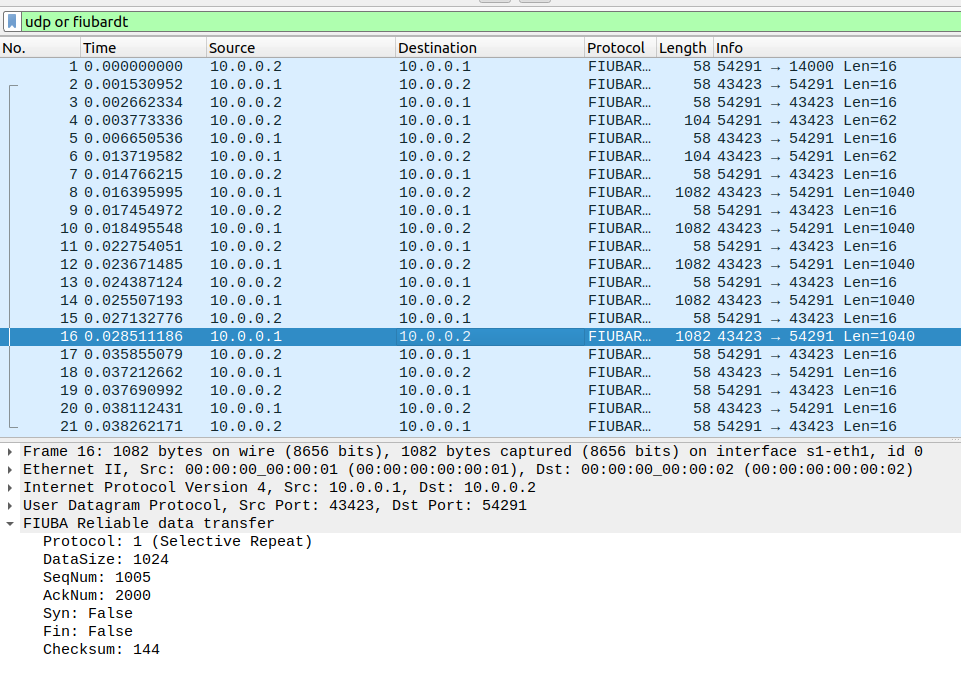
\includegraphics[width=15cm]{images/tests/t1/download/T1_3.3_download_SR_loss0.png}
                    \end{center}
                    \caption{Captura de wireshark del protocolo}
                \end{figure}
                \begin{figure}[H]
                    %\centering
                    \begin{center}
                    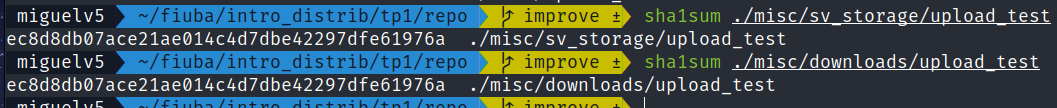
\includegraphics[width=15cm]{images/tests/t1/download/T1_3.4_download_SR_loss0.png}
                    \end{center}
                    \caption{Verificaci\'{o}n de SHA1 de los archivos}
                \end{figure}
            \end{itemize}
%%%%%%%% PACKET LOSS 10 %%%%%%%%%%%%%%%%%%%%%%%%%%%%%%%%%%%%%%%%%%%%%%%%%%%%%%%%%%%
\newpage
        \item \textbf{packet loss = 10}:
            \begin{figure}[H]
                %\centering
                \begin{center}
                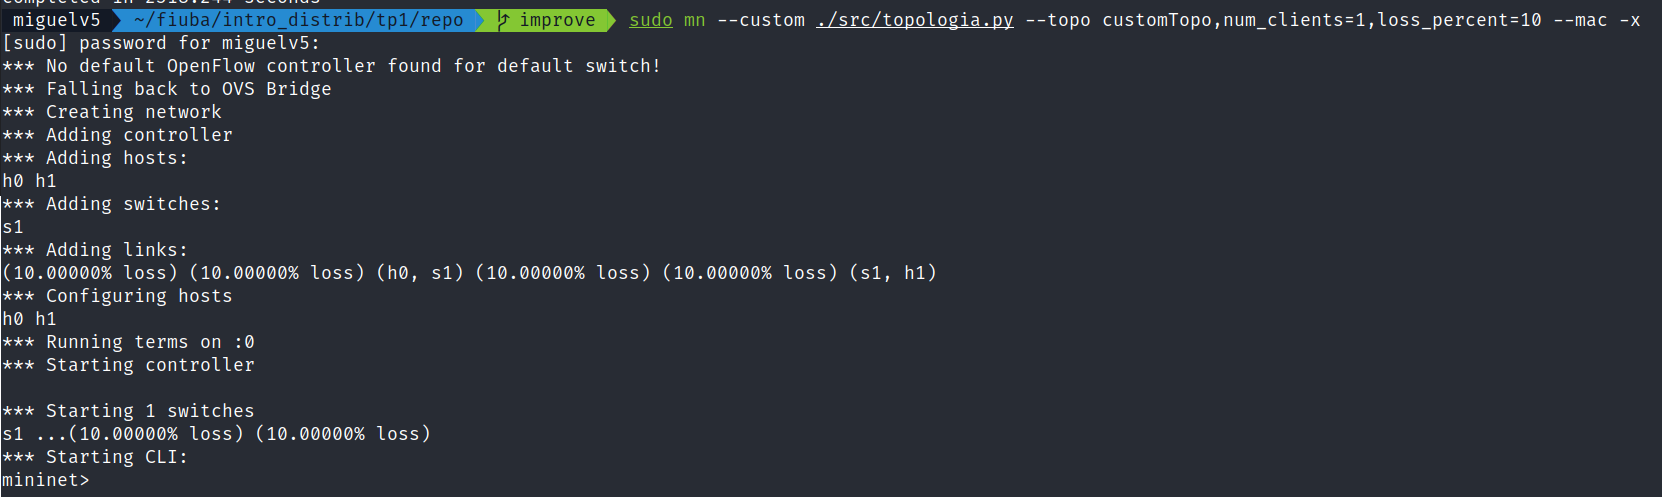
\includegraphics[width=18cm]{images/tests/t1/T1_loss10.png}
                \end{center}
                \caption{Mininet Topologia Packet loss $10\%$}
            \end{figure}
            \begin{itemize}
%%%%%%%% UPLOAD %%%%%%%%%%%%%%%%%%%%%%%%%%%
                    \item UPLOAD del archivo (Client $-->$ Server)
                        \begin{figure}[H]
                            %\centering
                            \begin{center}
                            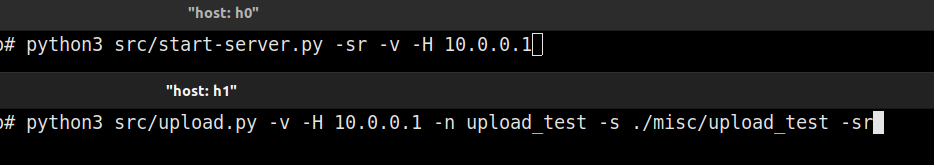
\includegraphics[width=18cm]{images/tests/t1/upload/T1_comandos_upload.png}
                            \end{center}
                            \caption{Comandos de ejecuci\'{o}n de servidor y cliente}
                        \end{figure}
                        \begin{figure}[H]
                            %\centering
                            \begin{center}
                            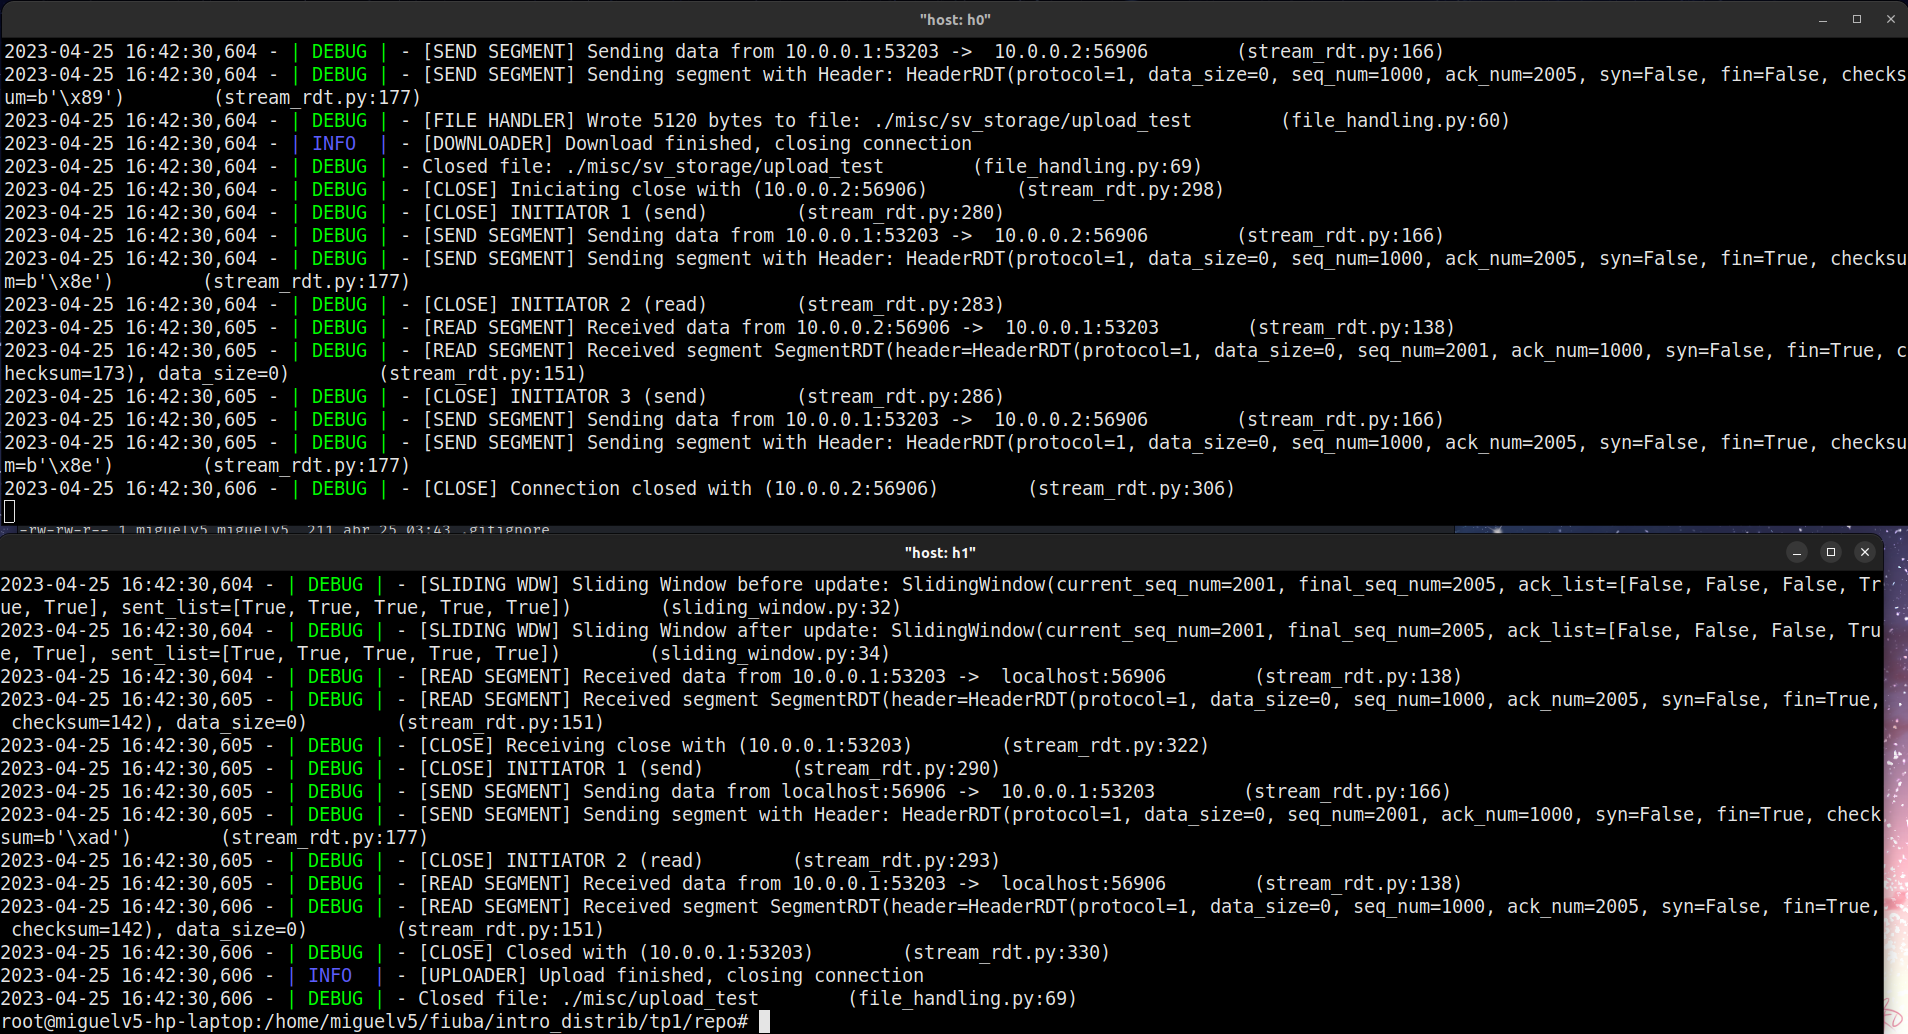
\includegraphics[width=18cm]{images/tests/t1/upload/T1_3.2_upload_SR_loss10.png}
                            \end{center}
                            \caption{Captura de comunicaci\'{o}n por linea de comandos}
                        \end{figure}
                        \begin{figure}[H]
                            %\centering
                            \begin{center}
                            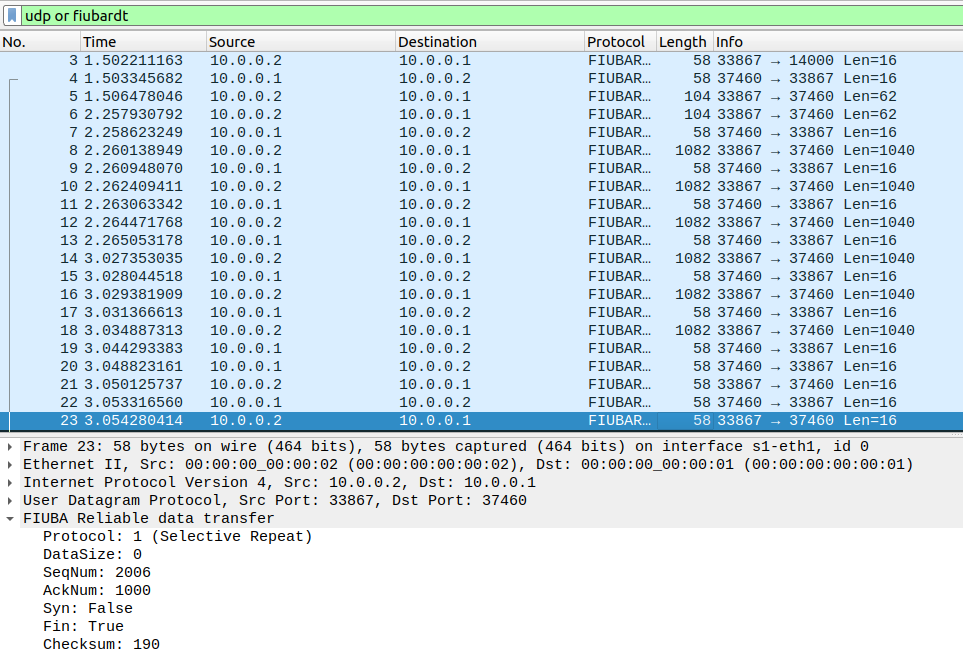
\includegraphics[width=15cm]{images/tests/t1/upload/T1_3.3_upload_SR_loss10.png}
                            \end{center}
                            \caption{Captura de wireshark del protocolo}
                        \end{figure}
                        \begin{figure}[H]
                        %\centering
                        \begin{center}
                        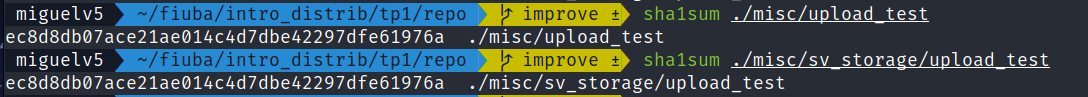
\includegraphics[width=15cm]{images/tests/t1/upload/T1_3.4_upload_SR_loss10.png}
                        \end{center}
                        \caption{Verificaci\'{o}n de SHA1 de los archivos}
                    \end{figure}
%%%%%%%% DOWNLOAD %%%%%%%%%%%%%%%%%%%%%%%%%
                    \item DOWNLOAD del archivo (Client $<--$ Server)
%%%%%%%% DOWNLOAD SELECTIVE REPEAT %%%%%%%%%
                        \begin{figure}[H]
                            %\centering
                            \begin{center}
                            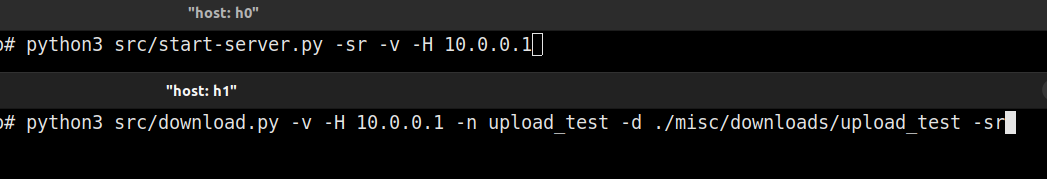
\includegraphics[width=18cm]{images/tests/t1/download/T1_comandos_download.png}
                            \end{center}
                            \caption{Comandos de ejecucci\'{o}n de servidor y cliente}
                        \end{figure}
                        \begin{figure}[H]
                            %\centering
                            \begin{center}
                            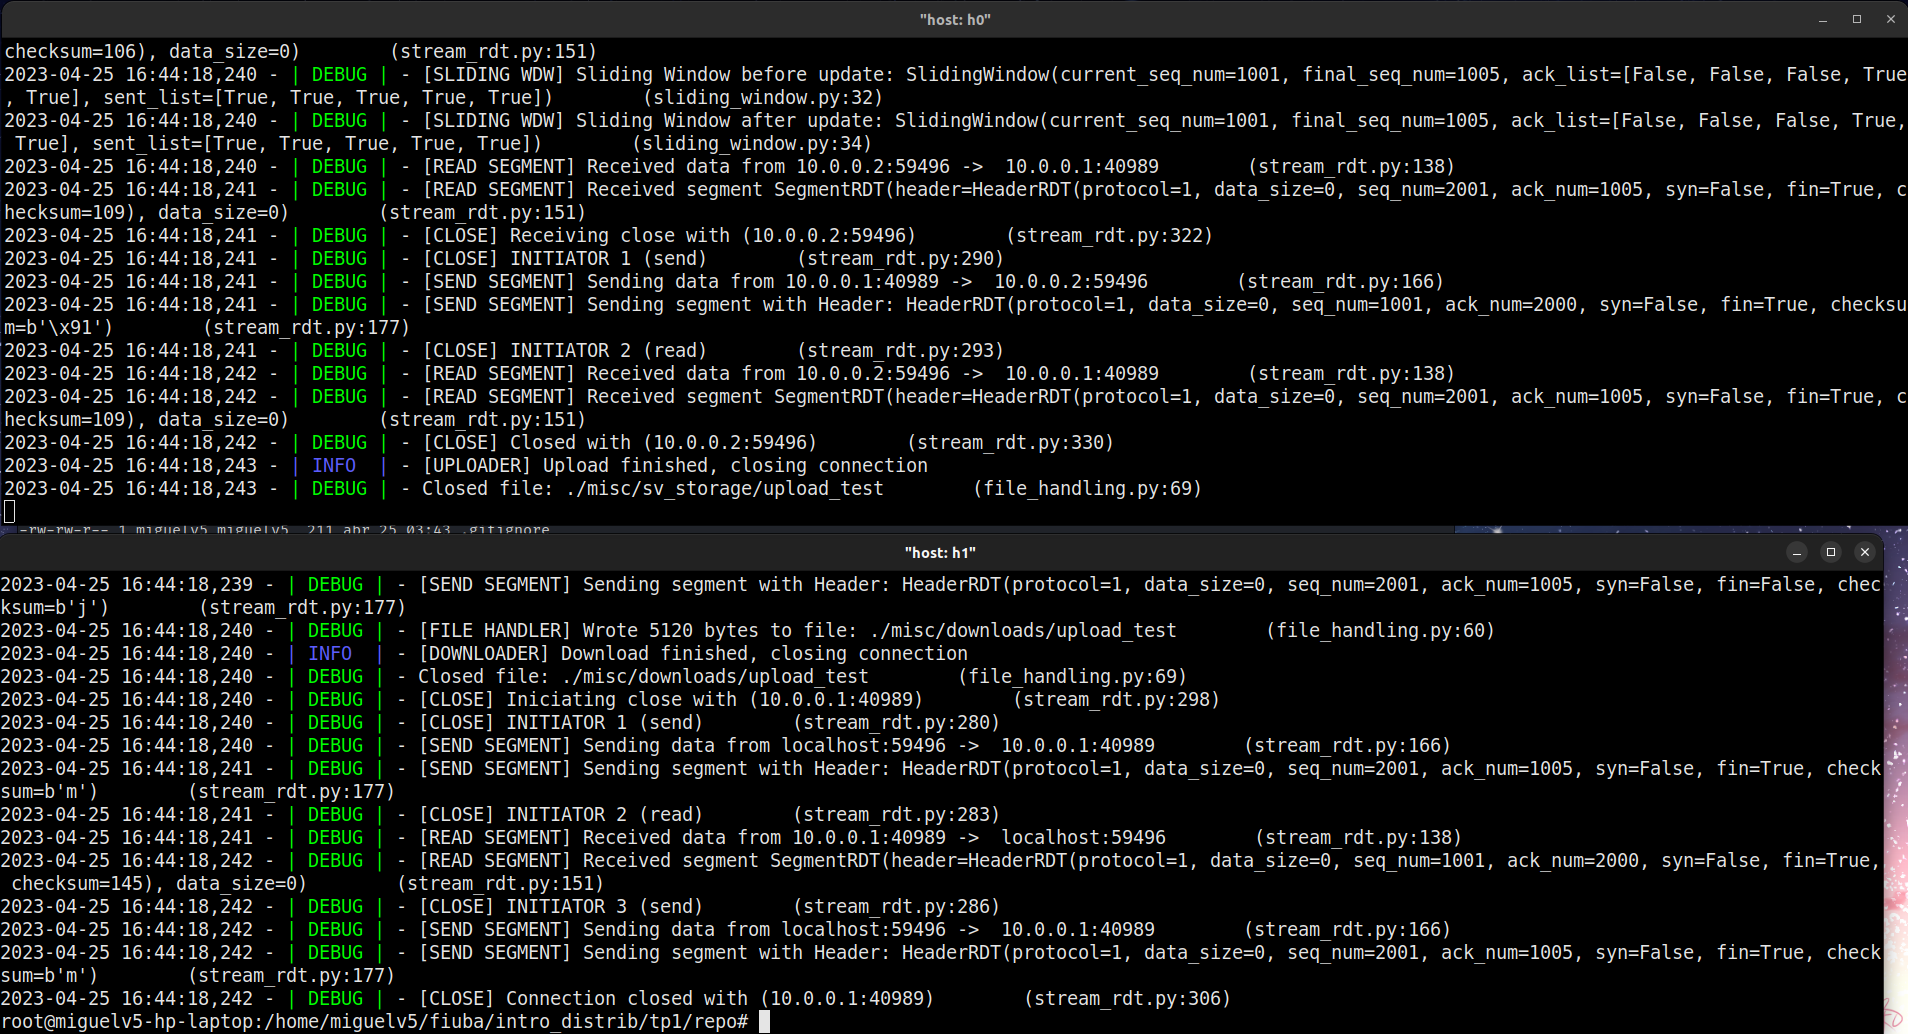
\includegraphics[width=18cm]{images/tests/t1/download/T1_4.2_download_SR_loss10.png}
                            \end{center}
                            \caption{Captura de comunicaci\'{o}n por linea de comandos}
                        \end{figure}
                        \begin{figure}[H]
                            %\centering
                            \begin{center}
                            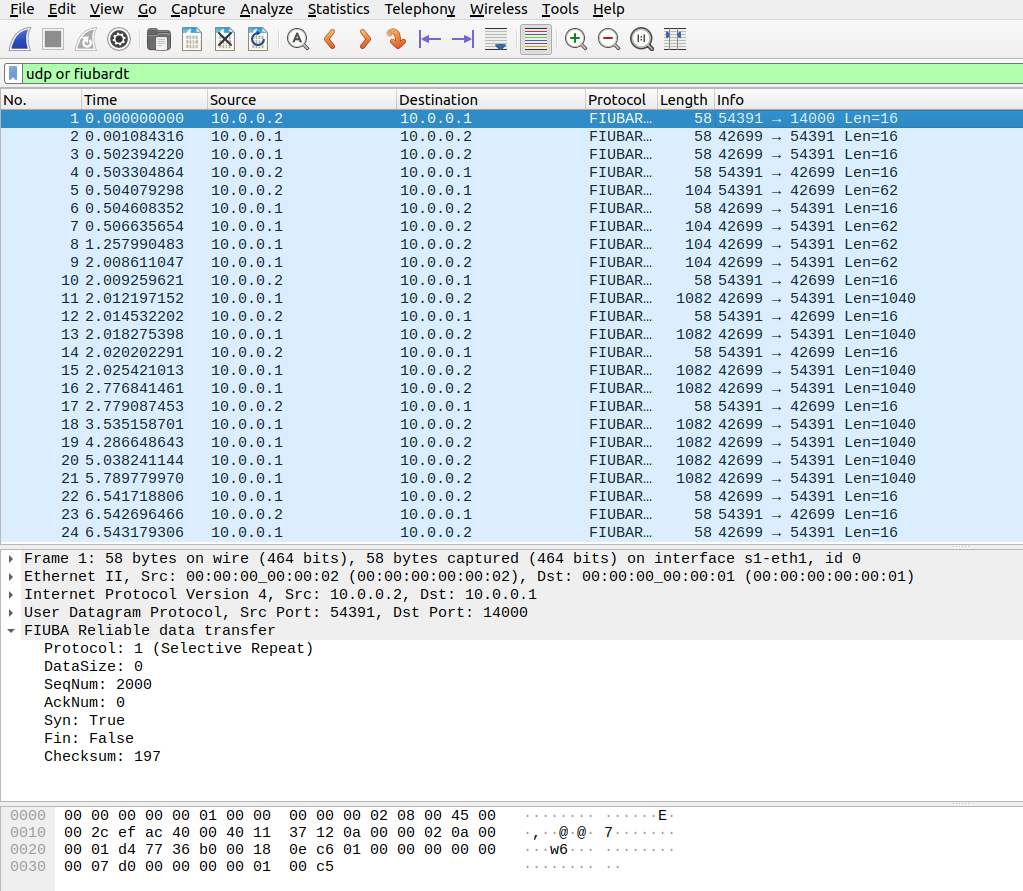
\includegraphics[width=15cm]{images/tests/t1/download/T1_4.3_download_SR_loss10.png}
                            \end{center}
                            \caption{Captura de wireshark del protocolo}
                        \end{figure}
                        \begin{figure}[H]
                        %\centering
                        \begin{center}
                        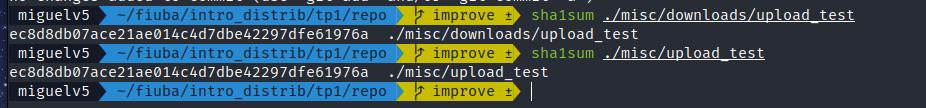
\includegraphics[width=15cm]{images/tests/t1/download/T1_4.4_download_SR_loss10.png}
                        \end{center}
                        \caption{Verificaci\'{o}n de SHA1 de los archivos}
                    \end{figure}
                \end{itemize}
    \end{itemize}


Para la correcta validación de las transferencias se utilizó el comando \textbf{sha1sum}. El comando sha1sum se encuentra en los sistemas Unix y permite identificar la integridad de un fichero mediante la comprobación del hash encodificado en \textbf{SHA-1}.

\newpage



\newpage

\section{Preguntas a responder}

\paragraph{Preguntas}

\begin{enumerate}
    \item Describa la arquitectura Cliente-Servidor.
    \item ¿Cuál es la función de un protocolo de capa de aplicación?
    \item Detalle el protocolo de aplicación desarrollado en este trabajo.
    \item La capa de transporte del stack TCP/IP ofrece dos protocolos: TCP y UDP. ¿Qué servicios proveen dichos protocolos? ¿Cuáles son sus características? ¿Cuando es apropiado utilizar cada uno?
\end{enumerate}

\paragraph{Respuestas}
\begin{enumerate}
    \item La arquitectura cliente-servidor es un modelo de red en el que los procesos de la aplicación se dividen en dos categorías: el cliente y el servidor. El servidor es un programa que espera las solicitudes de los clientes y responde a ellas. Por otro lado, el cliente es un programa que envía solicitudes al servidor y espera a que éste le devuelva una respuesta.
    
    En esta arquitectura, los servidores se ejecutan en máquinas dedicadas y están diseñados para atender solicitudes de múltiples clientes al mismo tiempo. Los clientes, por otro lado, pueden ser programas que se ejecutan en la misma máquina que el servidor o en máquinas remotas.
    
    Una de las características clave de la arquitectura cliente-servidor es que los clientes no interactúan directamente entre sí. En lugar de eso, cualquier comunicación entre clientes se realiza a través del servidor. Esto significa que el servidor actúa como un intermediario entre los clientes, lo que puede simplificar el diseño y la implementación de la aplicación.
    
    En la arquitectura cliente-servidor, la comunicación entre el cliente y el servidor se lleva a cabo mediante el intercambio de mensajes. Los clientes envían solicitudes al servidor en forma de mensajes, y el servidor responde a esas solicitudes enviando mensajes de respuesta. Estos mensajes pueden ser de diferentes tipos, como mensajes de solicitud, mensajes de respuesta, mensajes de confirmación, etc.
    
    Para que la comunicación cliente-servidor se realice correctamente, se utilizan varios protocolos. Los protocolos definen las reglas y el formato de los mensajes que se intercambian entre el cliente y el servidor, y también definen el comportamiento de los clientes y los servidores en diferentes situaciones.
    
    Entonces, la arquitectura cliente-servidor es un modelo de red en el que los procesos de la aplicación se dividen en dos categorías: el cliente y el servidor. Los clientes envían solicitudes al servidor y esperan a que éste les devuelva una respuesta. El servidor, por su parte, está diseñado para atender solicitudes de múltiples clientes al mismo tiempo y actúa como intermediario entre los clientes. La comunicación entre el cliente y el servidor se lleva a cabo mediante el intercambio de mensajes, y se utilizan varios protocolos para garantizar una comunicación efectiva.
    \item La función principal de un protocolo de capa de aplicación es proporcionar servicios de comunicación a las aplicaciones que se ejecutan en diferentes hosts en la red y definir las reglas y los formatos para el intercambio de datos entre las aplicaciones.
    
    El objetivo principal de un protocolo de capa de aplicación es proporcionar servicios de comunicación a las aplicaciones que se ejecutan en diferentes hosts en la red.
    
    En otras palabras, la capa de aplicación es la capa superior del modelo de referencia OSI y TCP/IP, y está diseñada para proporcionar una interfaz entre las aplicaciones y la red subyacente. Los protocolos de capa de aplicación se encargan de los detalles de la comunicación de extremo a extremo, incluyendo la codificación, el formato y el procesamiento de los mensajes enviados y recibidos por las aplicaciones.
    
    Además de proporcionar servicios de comunicación a las aplicaciones, los protocolos de capa de aplicación también definen las reglas y los formatos para el intercambio de datos entre las aplicaciones. Por ejemplo, algunos protocolos de aplicación comunes incluyen el protocolo HTTP para la transferencia de documentos web, el protocolo FTP para la transferencia de archivos y el protocolo SMTP para el correo electrónico.

    En nuestro caso particular, como se detalla anteriormente en la sección de Implementación, se define nuestro protocolo de aplicación cuando se hace referencia exclusivamente al envío de $"ApplicationHeaderRDT"$ con datos de archivos subsecuentes.

    \item El protocolo de aplicación del trabajo hace uso de un encabezado especifico que denota los siguientes campos:
    \begin{itemize}
        \item El nombre del archivo
        \item El tamaño del archivo
        \item El tipo de interacción, \textit{upload} o \textit{download}
    \end{itemize}
    Estos campos se utilizan en la capa de aplicación para reunir los datos de los segmentos y corroborar su tamaño final. A la capa de aplicación le llegan datos ordenados de la capa de transporte de a partes, para que luego vaya escribiendo el archivo abierto.
    El protocolo que define la secuencia de envío de mensajes de nuestra aplicación se encuentra definido en la sección Implementación de este informe.
    \item TCP (Transmission Control Protocol) y UDP (User Datagram Protocol) son los dos protocolos ofrecidos por la capa de transporte del stack TCP/IP. Ambos protocolos tienen diferentes características y se utilizan en diferentes situaciones.
    
    TCP es un protocolo orientado a la conexión que proporciona una comunicación confiable y ordenada de extremo a extremo. TCP asegura que todos los datos se envíen y se reciban correctamente, y en el orden correcto. Para lograr esto, TCP utiliza un sistema de confirmación y retransmisión de paquetes que garantiza que los datos lleguen a su destino sin errores. TCP es ampliamente utilizado por aplicaciones que requieren una transmisión de datos confiable y en orden, como la transferencia de archivos y el correo electrónico.
    
    Por otro lado, UDP es un protocolo sin conexión que proporciona una comunicación no confiable y no ordenada de extremo a extremo. A diferencia de TCP, UDP no utiliza confirmaciones ni retransmisiones de paquetes, por lo que no se garantiza que los datos lleguen a su destino sin errores o en el orden correcto. UDP se utiliza en situaciones en las que la velocidad y la eficiencia son más importantes que la confiabilidad, como en la transmisión de video y audio en tiempo real.
    
\end{enumerate}


\newpage

\section{Dificultades encontradas}

Durante el desarrollo e implementación del protocolo y las distintas capas, nos encontramos con diferentes dificultades.

Una de estas dificultades estuvo asociada la las pruebas de transferencia de archivos. Cuando se hacen este tipo de pruebas con un porcentaje de pérdida de paquetes, puede ser muy difícil reproducir errores específicos. Esto se debe a que el porcentaje de pérdida ejerce un peso probabilístico sobre la pérdida de cada paquete individual. Además, es difícil hacer estas pruebas con múltiples clientes conectados al servidor al mismo tiempo, ya que esto agrega un factor de incertidumbre inherente a la concurrencia, lo que limita la validez de la prueba.

Para abordar este problema, se decidió implementar un comportamiento similar al del protocolo TCP mediante la creación de un \textit{three-way-handshake} para establecer una conexión directa con un \textit{socket} específico del servidor.

Adicionalmente, durante el proceso de implementación, surgieron varios desafíos relacionados con la configuración de los parámetros del sistema, como los \textit{timeouts} para cada lectura y la cantidad de intentos permitidos después de dichos \textit{timeouts}. Factores como la pérdida del primer paquete del \textit{handshake} o la pérdida del último paquete del \textit{handshake} también complicaron las cosas. Además, los retrasos no previstos, como los causados por la lectura y escritura de archivos en disco durante las transferencias, obligaron a ajustar los parámetros para evitar que los \textit{timeouts} se excedieran en gran medida.

Para todo lo anterior fue de mucha utilidad la utilización de Wireshark para ver de forma sencilla el orden y todos los factores asociados a cada transmisión particular, y sumandole el disector personalizado facilitó aun más este proceso de análisis.


\newpage

\section{Conclusiones}
Este trabajo logró desarrollar una solución eficiente y confiable para la transferencia de datos entre dispositivos en una red simulada con Mininet. La arquitectura implementada se basó en los principios de la arquitectura cliente-servidor, utilizando sockets en Python para la comunicación entre hosts.

Para corroborar el correcto envio y recepcion se agrego packet loss a la red simulada 
y aunque se encontraron dificultades en el manejo de paquetes y segmentos, se aplicaron técnicas de control de flujo y control de errores, como Stop-and-wait y Selective Repeat, para garantizar la correcta transferencia de los archivos y verificacion de headers mediante Cyclic Redundancy Checks.

En general, este trabajo permitió aplicar los conceptos de la materia y las notas de las clases a un problema real en el mundo de redes. La implementación de esta solución fue una oportunidad valiosa para poner en práctica los conocimientos adquiridos y enfrentar los desafíos que impone una implementación de una solución eficiente y confiable de transferencia de datos en una red de computadoras, y la complejidad que poseen los protocolos de capa de transporte que garantizan RDT (Reliable Data Transfer) por sobre el protocolo UDP que no ofrece ninguna ganrantía del estilo.


Adicionalmente permitió el aprendizaje de herramientas como Wireshark para realizar un análisis de disección de cada paquete que se registra como transferido por la red.

\includepdf[pages=1, scale=0.98, pagecommand={\section{Enunciado} \vspace{0.1ex}}]{enunciado.pdf}
\includepdf[pages={2-}, scale=0.98]{enunciado.pdf}

\end{document}